\section{Introduction}
\label{sec:introduction}

Large language models (LLMs) increasingly rely on inference-time reasoning strategies that generate, revise, and aggregate multiple candidate solutions. Chain-of-thought prompting encourages models to expose intermediate reasoning \cite{wei2022cot}, self-consistency aggregates multiple independently sampled reasoning paths \cite{wang2023selfconsistency}, and iterative refinement methods allow a model to reconsider its own output through feedback \cite{madaan2023selfrefine,shinn2023reflexion}. Multi-agent debate (MAD) extends this idea from repeated reasoning within one model to interaction among several agents: each agent first proposes a solution, observes peer arguments, and revises its answer over multiple rounds \cite{du2023multiagent,liang2024debate,chen2024reconcile}. This paradigm is appealing because disagreement can expose mistakes that isolated reasoning would miss, while agreement among several agents appears to provide a natural signal of confidence.

Yet agreement is only useful when the evidence underlying it remains sufficiently independent. This distinction is easy to overlook in LLM debate. Unlike independent samples in classical ensemble reasoning, later-round votes are generated after agents have observed one another. An answer supported by three agents may therefore arise in fundamentally different ways: three agents may have reached it independently, or one agent may have proposed it and the others subsequently adopted it. These outcomes have the same vote count but different informational provenance. Social influence, sycophancy, and persuasion in interacting LLMs further complicate the interpretation of consensus \cite{zhang2024collaboration,sharma2024sycophancy,smit2024mad}. Consequently, the central reliability question is not merely \emph{how many agents agree}, but \emph{where that agreement came from}.

We begin by showing that this distinction matters because multi-agent debate is not information preserving. A correct hypothesis may appear during the interaction and nevertheless disappear before the final vote when its supporting agents revise toward an incorrect alternative. We refer to this phenomenon as \emph{correct-hypothesis extinction}. Across our core experiments, preserving the complete hypothesis history raises candidate recall from approximately $0.64$ to $0.76$, revealing substantial information that a conventional final-round decision discards. More broadly, the pre-debate independent decision outperforms the debated final majority on four of five core benchmarks, showing that additional interaction is not uniformly constructive. These observations motivate a shift from treating debate solely as an answer-improvement process to treating it as a dynamic information system in which useful hypotheses can be created, propagated, and destroyed.

A natural response is to predict which debates are about to fail and intervene selectively. We find, however, that detecting failure and predicting the value of intervention are fundamentally different problems. Extinction itself is predictable: a hazard model achieves an ROC--AUC of approximately $0.73$, and an oracle intervention analysis exposes a large potential improvement of $16.5$ percentage points. Nevertheless, across five pre-registered attempts using increasingly rich pre-intervention signals, we cannot reliably identify which individual debates will actually benefit from intervention. Cheap structural features, semantic representations, active self-diagnosis, placebo-controlled response probes, and mid-debate trajectories all fail the same benefit-prediction gate. Thus, \emph{failure predictability does not imply intervention actionability}. Rather than continuing to search for a controller that targets individual debates, we address the information loss structurally.

Our resulting view is \emph{hypothesis preserving}. Instead of allowing an agent's latest answer to overwrite earlier candidates, we retain the set of hypotheses that appeared throughout the frozen debate history and attach a provenance record to each candidate. This record captures how the hypothesis entered and survived the interaction, including its number of independent round-$0$ origins, cumulative support, persistence, and subsequent social adoption. The resulting representation separates two quantities that ordinary majority voting conflates: the \emph{magnitude} of consensus and the \emph{origin} of consensus. The analysis is performed post hoc over frozen debate transcripts and requires no additional LLM calls; an end-to-end live non-destructive debate protocol is left for future work.

This provenance view reveals the central empirical finding of the paper: \emph{not all consensus is equally informative}. First, hypothesis provenance is strongly associated with correctness across model families, task families, model scales, and agent counts. More importantly, this relationship cannot be explained merely by total support. The number of independent origins and total support are strongly correlated ($r\approx0.83$), so we explicitly compare hypotheses at matched levels of total consensus. Holding total support fixed, an additional independent round-$0$ supporter remains strongly associated with correctness, with a partial log-odds coefficient of $\beta_{\mathrm{ind}}=0.649$ and a clustered-bootstrap $95\%$ confidence interval of $[0.565,0.737]$. A decomposition of support gives a coefficient of $1.035$ for independently generated support versus $0.386$ for socially inherited support, corresponding to approximately $2.68\times$ larger conditional association per vote. The effect remains significant on seven of eight valid benchmarks and all five evaluated configurations, spanning model families from roughly $3$B to $14$B parameters and agent populations of $N\in\{3,5\}$. StrategyQA is the principal boundary case.

The matched-support comparison makes the phenomenon especially clear. For hypotheses with total support $n_{\mathrm{sup}}=4$, empirical correctness rises from $0.21$ when no support is independently generated to $0.44$, $0.66$, and $0.74$ as the number of independent origins increases from one to three. Comparable monotonic patterns appear at larger support levels. Importantly, we interpret this result as an \emph{epistemic signal}, not as a causal effect: independently generated agreement is associated with correctness after controlling for total consensus, but the observational debate logs do not establish that increasing independent support would itself cause an answer to become correct.

This mechanism also clarifies why provenance-aware reranking produces real but non-universal decision gains. Total support already captures much of the same information as independent support; adding provenance origin to raw support improves candidate-level AUC by only approximately $0.007$. Thus, a strong conditional relationship need not translate into a large incremental ranking advantage. Consistent with this explanation, a frozen provenance-aware selector improves over the deployed final majority in regimes where two conditions are simultaneously satisfied: provenance must discriminate correct from incorrect hypotheses, and a recoverable correct hypothesis must be available in the preserved pool. Under these conditions the selector improves pooled accuracy by approximately $3.2$ percentage points with no additional LLM calls and also outperforms the influence-based voting rule inherited from our earlier work. Outside these regimes, the gain is statistically indistinguishable from zero rather than universally positive. We therefore treat provenance-aware selection as a downstream application of the mechanism, not as the paper's central claim.

These results also refine an influence-centered view of multi-agent debate. Existing work has investigated communication topology, agent collaboration, persuasion, sycophancy, and which agents exert disproportionate influence over a group \cite{li2024sparse,zhang2024collaboration,sharma2024sycophancy}. Influence is important for describing how opinions propagate, but it does not determine whether the propagated hypothesis is correct. Our experiments show that an influence-aware voting rule can underperform plain majority voting, whereas hypothesis-level provenance remains strongly associated with correctness. The relevant unit of analysis is therefore not only the \emph{agent} that leads the debate, but the \emph{evidential history} of the hypothesis being selected.

The contributions of this work are fivefold:
\begin{itemize}
    \item \textbf{Correct-hypothesis extinction.} We identify and quantify a failure mode in which a correct hypothesis is generated during debate but disappears before the final decision, exposing substantial recoverable information that conventional final-round aggregation discards.
    \item \textbf{Failure predictability is not intervention-benefit predictability.} We show that extinction can be detected and has a large oracle intervention ceiling, yet five increasingly informative pre-registered benefit-prediction attempts fail to identify which individual debates should be targeted, motivating a structural rather than selective remedy.
    \item \textbf{Hypothesis preservation and provenance.} We formulate a non-destructive representation of frozen debate histories in which previously generated hypotheses are retained and annotated by their origin, support, persistence, and adoption history, enabling reliability analysis without additional LLM inference.
    \item \textbf{Consensus is not epistemically homogeneous.} At matched total support, independently generated agreement carries substantially more correctness signal than socially inherited agreement. This relationship is robust across seven of eight benchmarks and all five model/agent configurations, including a $14$B anchor and $N=5$ debates.
    \item \textbf{From mechanism to conditional decision utility.} We show that provenance-aware reranking can convert part of the preserved headroom into accuracy gains at zero additional LLM cost, while identifying the conditions under which such gains are possible and explaining why they are necessarily regime dependent.
\end{itemize}

Taken together, our results suggest a different principle for reliable collective reasoning with LLMs: consensus should not be treated as a homogeneous count of votes. Reliability depends not only on how much agreement exists, but also on how that agreement was formed. Preserving candidate hypotheses and tracking their epistemic provenance provides a way to distinguish independently corroborated evidence from socially inherited consensus, moving the analysis of multi-agent reasoning beyond influence and toward the origin of collective belief.

\section{Related Work}
\label{sec:related_work}

\subsection{Inference-Time Reasoning and Self-Refinement}
\label{subsec:rw_reasoning}

A broad family of inference-time methods improves LLM reasoning by generating additional intermediate computation rather than changing model parameters. Chain-of-thought prompting elicits explicit reasoning trajectories \cite{wei2022cot}, while self-consistency samples multiple trajectories and selects an answer through agreement across independently generated chains \cite{wang2023selfconsistency}. Self-Refine repeatedly revises an answer using model-generated feedback \cite{madaan2023selfrefine}, and Reflexion equips language agents with verbal feedback that can influence subsequent attempts \cite{shinn2023reflexion}. These approaches establish that repeated inference can expose and correct errors, but they differ from multi-agent debate in an important respect: agreement obtained from independently sampled trajectories has a clearer interpretation than agreement obtained after agents have observed and influenced one another. Our work focuses on this loss of independence and asks whether the provenance of agreement changes how strongly consensus should be trusted.

\subsection{Multi-Agent Debate and Collaborative LLM Reasoning}
\label{subsec:rw_mad}

Multi-agent debate has emerged as a prominent strategy for collective LLM reasoning. Du et al. demonstrate that iterative exchange among multiple language-model instances can improve factuality and reasoning \cite{du2023multiagent}. Subsequent work explores divergent debate to increase reasoning diversity \cite{liang2024debate}, round-table consensus across heterogeneous models \cite{chen2024reconcile}, sparse communication topologies that reduce interaction cost \cite{li2024sparse}, and broader design principles and interventions for multi-LLM debate \cite{estornell2024multillm}. General multi-agent frameworks such as CAMEL and AutoGen further illustrate the growing role of structured LLM-to-LLM interaction in reasoning and task execution \cite{li2023camel,wu2023autogen}.

Most of this literature evaluates debate through final-task accuracy, consensus, communication efficiency, or architectural choices. Such metrics implicitly treat the final state as the primary object of interest. Our work instead analyzes the \emph{trajectory of hypotheses} through the interaction. This exposes correct-hypothesis extinction: information can be present during debate and absent at the final vote. The distinction motivates hypothesis preservation and changes the relevant question from whether interaction reaches consensus to whether the system retains and correctly interprets the evidence that generated that consensus.

\subsection{Social Influence, Persuasion, and Sycophancy in LLM Agents}
\label{subsec:rw_social}

LLM agents do not exchange information neutrally. Social-psychological analyses show that collaboration patterns, agent roles, and interaction structures affect collective behavior \cite{zhang2024collaboration}. Sycophancy studies demonstrate that language models may align their responses with user or contextual preferences even when such agreement is not epistemically justified \cite{sharma2024sycophancy}. Evaluations of multi-agent debate similarly report that additional discussion is not uniformly beneficial and that debate strategy can substantially alter final performance \cite{smit2024mad}. More recent work has explicitly examined sycophancy mitigation in multi-agent consensus, reinforcing the concern that apparent agreement may partly reflect interaction dynamics rather than independent corroboration \cite{zhang2025consensagent}.

These studies motivate analyzing \emph{how} beliefs propagate, but influence and correctness are distinct. Agent-level centrality can identify who is followed, just as PageRank-like scores quantify structural importance in a directed interaction graph \cite{page1998pagerank}, yet a highly influential agent can propagate either a correct or an incorrect hypothesis. Our prior conference work used this agent-centric perspective to study who leads a debate; the present work shifts the unit of analysis from agents to hypotheses. We record whether support was independently generated or socially inherited and show that, even at equal total support, these forms of agreement carry different correctness signal. This establishes epistemic provenance as complementary to, and more directly relevant for reliability than, influence alone.

\subsection{Consensus, Independent Evidence, and the Wisdom of Crowds}
\label{subsec:rw_crowds}

The interpretation of consensus has long depended on assumptions about independence. Classical wisdom-of-crowds reasoning is strongest when individual judgments contain sufficiently independent information, so that errors can cancel rather than reinforce one another. Recent behavioral work likewise shows that convergence among independent and approximately unbiased informants can rationally signal competence and accuracy, while systematic shared biases weaken this inference \cite{pfander2025crowd}. This perspective is highly relevant to multi-agent LLM systems because later-round answers are explicitly conditioned on peer responses and therefore cannot be interpreted as independent observations.

Our results provide an LLM-specific operationalization of this principle. Rather than treating independence as an unobserved assumption, we track it directly through hypothesis provenance. We distinguish round-$0$ independent origins from support acquired after social exposure and compare them while holding total support fixed. The resulting difference is substantial: independently generated support remains strongly associated with correctness after controlling for raw consensus. In this sense, our work connects multi-agent LLM debate to the broader principle that the reliability of collective agreement depends on the dependence structure of the evidence producing it.

\subsection{Answer Selection, LLM-as-a-Judge, and Reliability Aggregation}
\label{subsec:rw_selection}

A separate line of work studies how to select among multiple model outputs. Self-consistency uses answer frequency over sampled reasoning paths \cite{wang2023selfconsistency}, while heterogeneous-agent systems frequently use majority voting, confidence weighting, or consensus-based aggregation \cite{chen2024reconcile,estornell2024multillm}. LLM-as-a-Judge methods instead ask a capable model to evaluate candidate responses directly; MT-Bench and Chatbot Arena helped establish the usefulness, as well as the biases and limitations, of this paradigm \cite{zheng2023judging}. In multi-agent settings, however, an external judge introduces additional inference cost and may solve the underlying problem more effectively than it discriminates among imperfect candidates.

Our approach differs from both answer-frequency aggregation and external judging. We exploit metadata already contained in the debate trajectory and therefore add no new LLM calls. More importantly, the provenance analysis is not introduced merely as a new scoring heuristic. Its primary role is explanatory: it reveals that equal consensus counts can encode different amounts of epistemic evidence. The resulting selector is intentionally treated as a downstream application, and we characterize rather than hide its applicability boundary. This separates the near-universal mechanism---independent provenance carries more correctness signal---from the more conditional question of whether that signal yields additional end-task accuracy over a strong consensus baseline.

\subsection{Positioning of This Work}
\label{subsec:rw_positioning}

The above literature reveals three unresolved gaps. First, existing MAD evaluations largely focus on final answers and therefore do not explicitly quantify correct hypotheses that appear and later disappear. Second, work on collaboration and influence explains how agents affect one another but does not determine whether socially propagated agreement should carry the same epistemic weight as independently generated agreement. Third, aggregation methods usually operate on the magnitude of support or on an external evaluator, without explicitly modeling the origin of that support. We address these gaps through a unified trajectory-level analysis: we quantify correct-hypothesis extinction, preserve the full candidate history, attach provenance to each hypothesis, and test whether the origin of agreement remains informative after controlling for total consensus. The resulting finding---that independently generated consensus carries substantially more correctness signal than socially inherited consensus at matched support---is the central distinction between our approach and prior influence-, consensus-, or judge-based methods.


\section{Problem Formulation}
\label{sec:problem_formulation}

This section fixes notation and defines the two objects the paper studies: the \emph{extinction} of a
correct hypothesis during debate, and the \emph{epistemic provenance} of the agreement that supports a
hypothesis. Throughout, we separate the deployed debate protocol, which generates the transcripts, from
our post-hoc analysis, which reads them; the analysis introduces no new model calls. The complete
experimental protocol is deferred to Appendix~\ref{app:protocol}.

\subsection{Multi-Agent Debate as Sequential Belief Revision}
\label{subsec:mad_formulation}

Let $\mathcal{A}=\{a_1,\dots,a_N\}$ be a set of $N$ heterogeneous LLM agents. Given a question $q$ drawn
from a benchmark $\mathcal{D}$ with gold answer $y^\star(q)$, the agents debate for up to $T$ synchronous
rounds. We write $x_i^{(r)}$ for the answer proposed by agent $a_i$ in round $r$, and
$\bar{x}=\mathrm{norm}(x)$ for a normalized answer, so that surface variants of the same answer are
treated as identical. At round $0$ each agent answers \emph{independently},
$x_i^{(0)}=a_i(q)$, with no knowledge of its peers. In every subsequent round the agents revise
\emph{simultaneously}, each conditioning on the previous round's answers of all peers:
\begin{equation}
x_i^{(r)} \;=\; a_i\!\Big(q,\; x_i^{(r-1)},\; \{x_k^{(r-1)}\}_{k\ne i}\Big),\qquad r\ge 1 .
\end{equation}
The debate stops early upon consensus and otherwise runs to round $T$. The deployed system returns the
majority answer over the agents' final responses,
$\hat{y}_{\mathrm{maj}}(q)=\arg\max_{c}\sum_{i}\mathbb{1}[\bar{x}_i^{(T)}=c]$, with ties broken
deterministically. This synchronous, peer-symmetric protocol is what makes belief revision --- and hence
provenance --- attributable: a change at round $r$ can be ascribed to what an agent saw at round $r-1$.

\subsection{Hypotheses and Debate Trajectories}
\label{subsec:hypothesis_trajectories}

We treat each distinct normalized answer value that appears in a debate as a \emph{hypothesis} $h$. Its
round-$r$ supporter set and the round-$r$ hypothesis set are
\begin{equation}
S^{(r)}(h)=\{\,i : \bar{x}_i^{(r)}=h\,\},\qquad
H^{(r)}=\{\,\bar{x}_i^{(r)} : i=1,\dots,N\,\}.
\end{equation}
A vanilla debate reports only the \emph{final pool} $H^{\mathrm{fin}}=H^{(T)}$. We contrast it with the
\emph{history pool} $H^{\mathrm{hist}}=\bigcup_{r\le T}H^{(r)}$, the set of all hypotheses that ever
appeared. The two coincide only if no hypothesis is ever abandoned; in general
$H^{\mathrm{fin}}\subseteq H^{\mathrm{hist}}$, and the difference is exactly the information a final-round
decision discards. The \emph{total support} of a hypothesis is its cumulative agent--round count,
$n_{\mathrm{sup}}(h)=\sum_{r=0}^{T}\lvert S^{(r)}(h)\rvert$, and its \emph{persistence} is the number of
rounds in which it is alive, $n_{\mathrm{per}}(h)=\lvert\{r : S^{(r)}(h)\ne\varnothing\}\rvert$.

\subsection{Correct-Hypothesis Extinction}
\label{subsec:extinction_definition}

A hypothesis becomes \emph{extinct} when it is present during the debate but absent from the final
decision. To quantify how often this destroys \emph{correct} information, we measure the probability that
the gold answer survives to the final round versus anywhere in the history:
\begin{equation}
\mathrm{CR}_{\mathrm{fin}}=\Pr\!\big(y^\star\in H^{\mathrm{fin}}\big),\quad
\mathrm{CR}_{\mathrm{hist}}=\Pr\!\big(y^\star\in H^{\mathrm{hist}}\big),\quad
\Delta\mathrm{CR}=\mathrm{CR}_{\mathrm{hist}}-\mathrm{CR}_{\mathrm{fin}} .
\label{eq:extinction}
\end{equation}
$\Delta\mathrm{CR}$ is the \emph{correct-hypothesis extinction rate}: the fraction of debates in which a
correct answer is generated and then forgotten. It is exactly the accuracy a perfect selector over a
preserved pool could recover over a perfect selector restricted to the final round, and it upper-bounds
the value of any preservation-based remedy.

\subsection{Epistemic Provenance of Agreement}
\label{subsec:provenance_definition}

Two hypotheses can carry identical total support yet have been produced in fundamentally different ways.
We decompose the support of $h$ by \emph{origin}. Its \emph{independent support} is the number of agents
that proposed it before observing any peer,
\begin{equation}
n_{\mathrm{ind}}(h)=\lvert S^{(0)}(h)\rvert ,
\end{equation}
and its \emph{socially inherited support} is the remaining, post-exposure support,
$n_{\mathrm{inh}}(h)=n_{\mathrm{sup}}(h)-n_{\mathrm{ind}}(h)$, accrued when an agent revises \emph{onto}
$h$ after seeing it held by a peer. We also record the round in which $h$ first appears,
$\mathrm{first}(h)=\min\{r:S^{(r)}(h)\ne\varnothing\}$. The tuple
$\big(n_{\mathrm{sup}},\,n_{\mathrm{ind}},\,n_{\mathrm{inh}},\,n_{\mathrm{per}},\,\mathrm{first}\big)$ is
the \emph{provenance} of a hypothesis. Majority voting sees only a coarse function of $n_{\mathrm{sup}}$;
our question is whether the finer, origin-aware decomposition carries additional correctness signal.

\subsection{Research Hypotheses}
\label{subsec:research_hypotheses}

The paper is organized around three pre-registered hypotheses of increasing sharpness:
\begin{itemize}
    \item[\textbf{H1}] \textbf{(Extinction).} Debate destroys correct answers it once held:
    $\Delta\mathrm{CR}>0$ (Eq.~\ref{eq:extinction}), and the pre-debate independent decision is not
    uniformly worse than the debated final decision.
    \item[\textbf{H2}] \textbf{(Provenance predicts correctness).} A hypothesis's own provenance predicts
    whether it is correct: $\Pr(\text{correct}\mid n_{\mathrm{ind}})$ and
    $\Pr(\text{correct}\mid n_{\mathrm{per}})$ are monotone increasing, with directional AUC above chance.
    \item[\textbf{H3}] \textbf{(Origin, at matched total support).} \emph{Holding total support fixed},
    independently generated agreement carries more correctness signal than socially inherited agreement:
    the partial effect of $n_{\mathrm{ind}}$ given $n_{\mathrm{sup}}$ is strictly positive.
\end{itemize}
The clause ``at matched total support'' in H3 is load-bearing. Independent support and total support are
strongly collinear (Pearson $r\approx0.83$), so H2 alone cannot separate \emph{how much} agreement exists
from \emph{how it was formed}; H3 is the mechanism behind H2, isolated by controlling for consensus
magnitude, not a restatement of it.


\section{Methodology}
\label{sec:methodology}

\subsection{Framework Overview}
\label{subsec:framework_overview}

Our method is a three-stage analysis of frozen debate transcripts --- \emph{preserve}, \emph{track
provenance}, and \emph{select} --- summarized in Figure~\ref{fig:framework}. We (i) retain every
hypothesis that appears in the debate rather than only the final round; (ii) annotate each retained
hypothesis with a provenance record describing how its support was formed; and (iii) optionally re-select
the final answer from the preserved pool using that record. All three stages operate post hoc on stored
transcripts and add \emph{no} LLM inference; the selection stage is therefore a drop-in replacement for
majority voting at zero marginal cost. We stress that the analysis is offline: we do not run a live
non-destructive debate, and we quantify what preservation and provenance \emph{could} recover from
transcripts a standard debate already produces.

\begin{figure}[t]
\centering
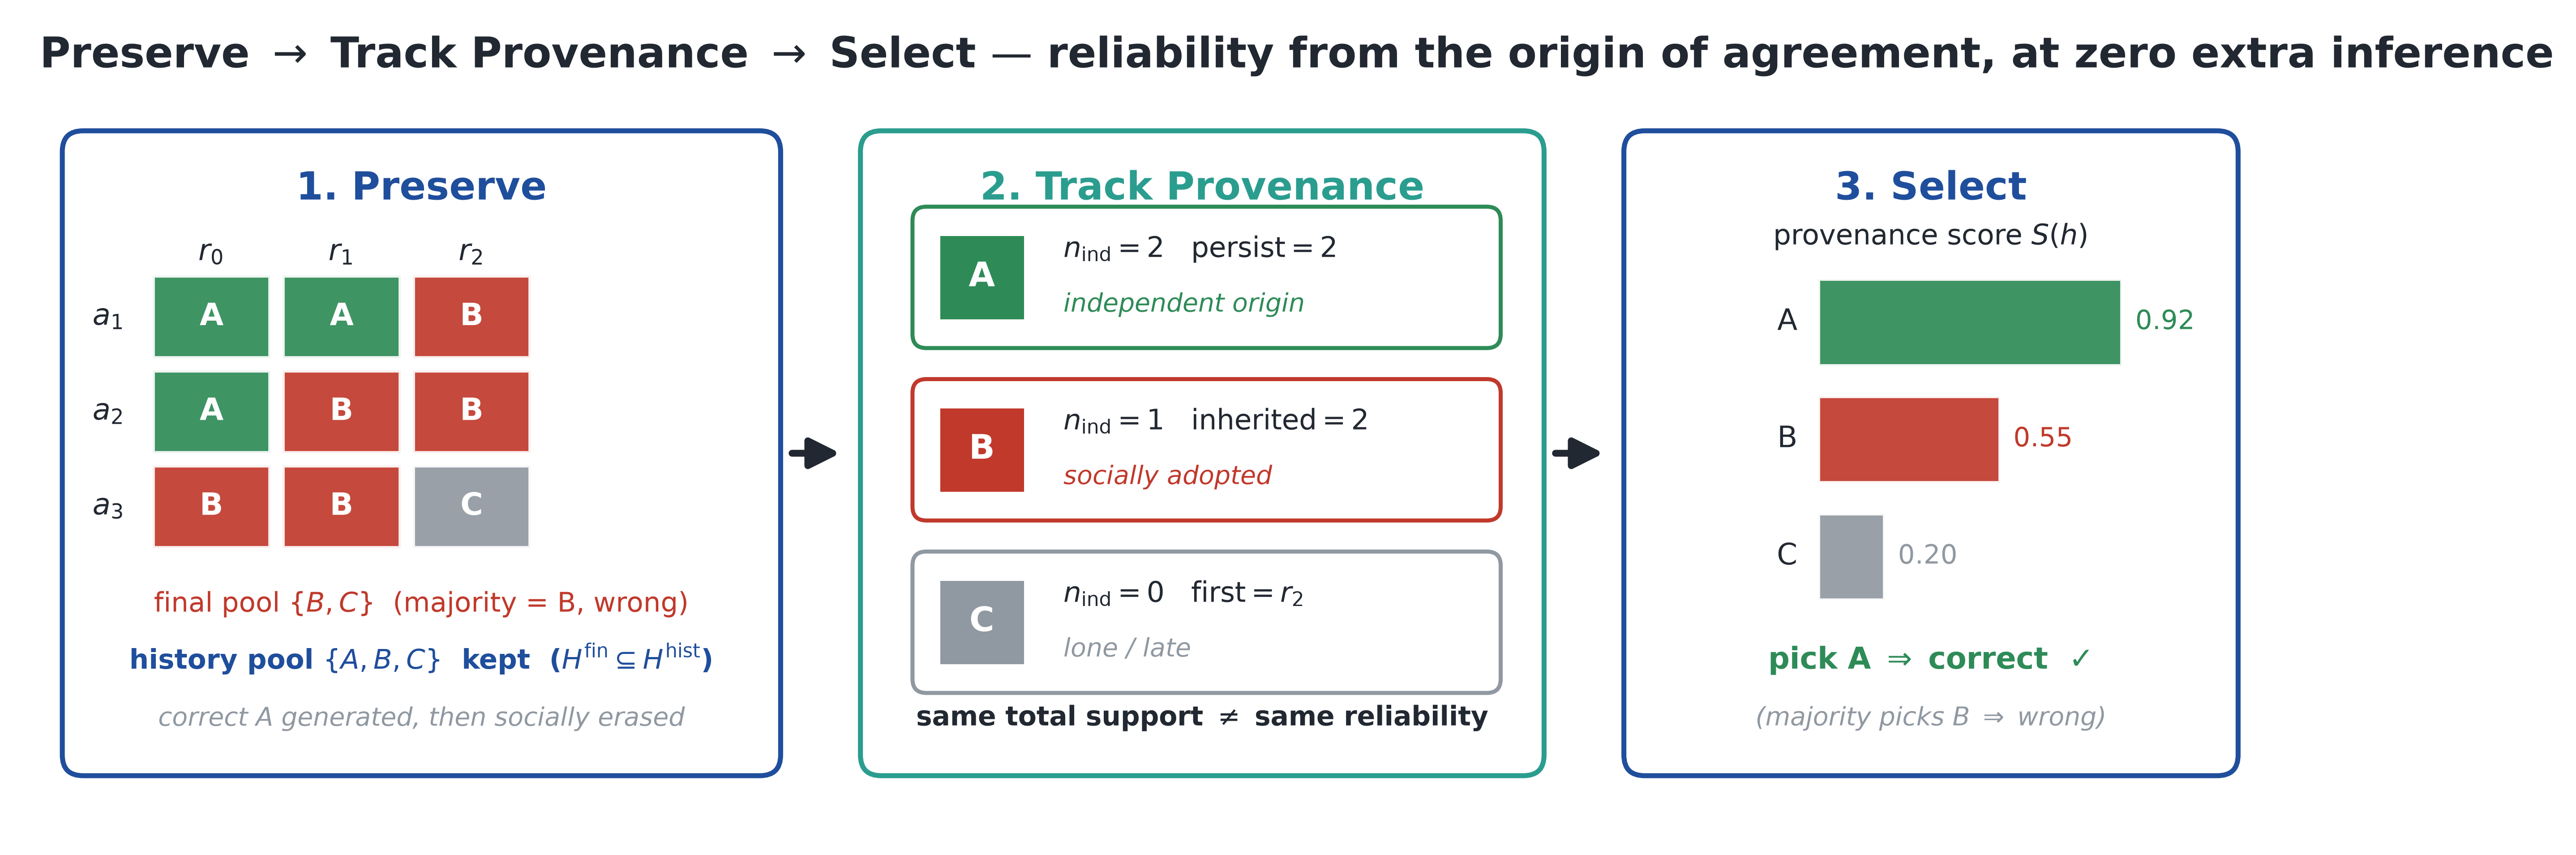
\includegraphics[width=\linewidth]{results/figures/fig1_framework.png}
\caption{\textbf{Preserve $\to$ Track Provenance $\to$ Select.} A standard debate destructively overwrites
earlier hypotheses and votes over the final round only; our analysis preserves the full history pool
($H^{\mathrm{fin}}\subseteq H^{\mathrm{hist}}$), attaches an origin-aware provenance record to each
candidate ($n_{\mathrm{ind}}$, persistence, first round), and re-selects the final answer by a provenance
score --- all without additional model calls. In the example, the correct hypothesis $A$ is generated
independently by two agents, socially erased by the final vote, but recovered because its independent
origin gives it the highest provenance score.}
\label{fig:framework}
\end{figure}

\subsection{Preserving the Hypothesis Space}
\label{subsec:hypothesis_preservation}

\paragraph{History-preserving candidate pool.}
\label{par:history_pool}
The core structural change is to replace the final-round pool $H^{\mathrm{fin}}$ with the history pool
$H^{\mathrm{hist}}=\bigcup_{r\le T}H^{(r)}$ as the candidate set from which the final answer is drawn.
Because a hypothesis, once generated, is never erased, the pool grows monotonically,
$H^{(0)}\subseteq H^{(0)}\!\cup H^{(1)}\subseteq\cdots\subseteq H^{\mathrm{hist}}$ --- a preservation
guarantee that a destructive debate lacks. This directly counters both extinction mechanisms
(Section~\ref{par:extinction_anatomy}): a correct hypothesis abandoned through social adoption or
self-error drift remains recoverable.

\paragraph{Reconstruction from frozen debate trajectories.}
\label{par:posthoc_reconstruction}
We reconstruct $H^{\mathrm{hist}}$ from stored transcripts using a robust answer extractor that recovers
answers hidden by response truncation (e.g.\ a \texttt{\textbackslash boxed\{\}} value cut off by the
token limit) and, crucially, \emph{censors} genuinely truncated generations so they cannot inflate recall.
Extraction, normalization, and correctness scoring are identical to those used for the deployed majority
vote, so the preserved pool is compared to the baseline on equal footing. Full extractor and scoring
details are given in Appendix~\ref{app:protocol}.

\subsection{Tracing the Provenance of Agreement}
\label{subsec:provenance_tracking}

\paragraph{Agent--round provenance graph.}
\label{par:provenance_graph}
For each hypothesis we read the transcript as a bipartite agent--round record: for every round $r$ and
agent $i$ we know whether $\bar{x}_i^{(r)}=h$, and whether that support is newly acquired
($\bar{x}_i^{(r)}=h\wedge \bar{x}_i^{(r-1)}\ne h$) or carried over. This record distinguishes
support that an agent \emph{originated} from support it \emph{adopted} after peer exposure.

\paragraph{Independent hypothesis origins.}
\label{par:independent_origins}
The independent support $n_{\mathrm{ind}}(h)=\lvert S^{(0)}(h)\rvert$ counts agents that proposed $h$ at
round $0$, before seeing any peer. It is the number of \emph{independent evidential paths} to $h$ and is
the central provenance quantity of the paper.

\paragraph{Socially inherited support.}
\label{par:inherited_support}
The inherited support $n_{\mathrm{inh}}(h)=n_{\mathrm{sup}}(h)-n_{\mathrm{ind}}(h)$ aggregates all
post-exposure support: votes that arose only after $h$ was visible in the debate. Two hypotheses can share
$n_{\mathrm{sup}}$ while differing sharply in the $n_{\mathrm{ind}}$/$n_{\mathrm{inh}}$ split.

\paragraph{Persistence across debate rounds.}
\label{par:persistence}
Persistence $n_{\mathrm{per}}(h)$ counts the rounds in which $h$ is alive; a hypothesis that survives
scrutiny across rounds is treated differently from one that flickers in a single round. Persistence is a
second, weaker provenance dimension that we report alongside origin but keep out of the headline claim.

\subsection{Representing Epistemic Provenance}
\label{subsec:provenance_representation}

Each candidate hypothesis is represented by the following features, all computable from the transcript
without gold labels.

\paragraph{Total support.}
\label{par:total_support}
$n_{\mathrm{sup}}(h)$, cumulative agent--round votes --- the quantity majority voting (approximately) uses.

\paragraph{Independent support.}
\label{par:independent_support}
$n_{\mathrm{ind}}(h)$, round-$0$ origins; the origin signal whose incremental value over $n_{\mathrm{sup}}$
we test.

\paragraph{Inherited support.}
\label{par:inherited_support_feature}
$n_{\mathrm{inh}}(h)$, post-exposure support; contrasted against $n_{\mathrm{ind}}$ per vote.

\paragraph{Temporal provenance.}
\label{par:temporal_provenance}
$n_{\mathrm{per}}(h)$ (persistence) and $\mathrm{first}(h)$ (first round of appearance); late-emerging
hypotheses are treated as suspect.

\subsection{Disentangling Consensus Magnitude from Consensus Origin}
\label{subsec:consensus_decomposition}

Because $n_{\mathrm{ind}}$ and $n_{\mathrm{sup}}$ are collinear ($r\approx0.83$), a raw association between
independent support and correctness could merely reflect that popular answers are correct. We therefore
test H3 with three complementary estimators that all hold total consensus fixed. All confidence intervals
are clustered bootstraps that resample at the (config, benchmark, question) level, so dependence among a
question's candidates and across seeds is respected; full inference details are in
Appendix~\ref{app:stats}.

\paragraph{Matched-total-support analysis.}
\label{par:matched_support}
Non-parametrically, we stratify candidates by $n_{\mathrm{sup}}$ and, within each stratum, report empirical
correctness as a function of $n_{\mathrm{ind}}$. If origin is inert once magnitude is fixed, correctness
should be flat within a stratum.

\paragraph{Independent--inherited support decomposition.}
\label{par:support_decomposition}
Parametrically, we fit a logistic model of correctness on the two origin components,
$\operatorname{logit}\Pr(\text{correct})=\beta_{\mathrm{ind}}\,n_{\mathrm{ind}}+\beta_{\mathrm{inh}}\,
n_{\mathrm{inh}}+\text{const}$, which yields the correctness value \emph{per vote} of each kind of support.

\paragraph{Controlled and fixed-effect estimation.}
\label{par:controlled_estimation}
Equivalently, we regress correctness on $n_{\mathrm{sup}}$ and $n_{\mathrm{ind}}$ jointly; the coefficient
on $n_{\mathrm{ind}}$ is then the extra correctness signal of an independent origin \emph{at matched total
support} (algebraically $\beta_{\mathrm{ind}}-\beta_{\mathrm{inh}}$ of the decomposition). We repeat the
estimate with benchmark and configuration fixed effects, and separately per benchmark and per
configuration, to check that the effect is not an artifact of task or ensemble composition.

\subsection{Provenance-Aware Hypothesis Selection}
\label{subsec:provenance_selection}

\paragraph{Candidate scoring.}
\label{par:candidate_scoring}
To turn the mechanism into a decision rule, we score each hypothesis in the preserved pool by
\begin{equation}
S(h)=w_1\,n_{\mathrm{ind}}(h)+w_2\,n_{\mathrm{per}}(h)+w_3\,n_{\mathrm{sup}}(h)-w_4\,\mathrm{first}(h),
\end{equation}
and return $\arg\max_h S(h)$. Weights are either fixed and equal (after standardizing features) or learned.

\paragraph{Cross-fitted estimation.}
\label{par:crossfit}
For the learned variant we fit logistic weights with group $k$-fold cross-fitting over questions, so no
candidate is ever scored by weights trained on its own question; reported accuracies are out-of-fold. This
prevents the selector from overfitting question-specific idiosyncrasies and makes the comparison to the
zero-parameter baselines fair.

\paragraph{Final decision rule.}
\label{par:decision_rule}
The selected answer replaces the deployed majority vote. Because scoring reads only stored provenance
features, the rule adds no LLM calls and is a strict post-processing step over any existing debate log.


\section{Experiments and Results}
\label{sec:experiments_results}

We report results as a single narrative: debate forgets correct answers
(\S\ref{subsec:extinction_results}); the natural levers for recovering them --- agent influence
(\S\ref{subsec:influence_insufficient}) and failure prediction
(\S\ref{subsec:prediction_actionability}) --- do not identify a useful action; so we attack the loss
structurally by preserving hypotheses and reading their provenance
(\S\ref{subsec:provenance_correctness}), which reveals the paper's central finding, that consensus is not
epistemically homogeneous (\S\ref{subsec:not_all_consensus_equal}); we then convert the mechanism into a
zero-cost decision rule whose gains are real but conditional
(\S\ref{subsec:decision_utility}), and confirm the scientific claims generalize
(\S\ref{subsec:generalization}). Unless noted, numbers are pooled over benchmarks $\times$ seeds under the
robust scorer, with clustered-bootstrap $95\%$ CIs over questions.

\subsection{Experimental Protocol}
\label{subsec:experimental_protocol}

We summarize the protocol here; Appendix~\ref{app:protocol} gives the full specification.

\paragraph{Benchmarks.}
\label{par:benchmarks}
The core experiments use five reasoning benchmarks spanning open-answer arithmetic (GSM8K), binary
strategic reasoning (StrategyQA), multiple-choice commonsense (CommonsenseQA), diverse hard tasks (BBH),
and adversarial factuality (TruthfulQA), with $500$ questions per benchmark $\times$ $5$ seeds. For the
generalization and provenance analyses we add three further multiple-choice benchmarks (AQuA, MMLU, ARC),
for eight benchmarks in total.

\paragraph{Models and agent configurations.}
\label{par:model_configs}
The base ensemble (\textsc{E\_orig}) is three peer agents with distinct personas
(\emph{careful}, \emph{skeptic}, \emph{bigpicture}) backed by three different open-weight models
(\texttt{qwen2.5:3b}, \texttt{phi4-mini}, \texttt{llama3.2:3b}). To probe generalization we vary the
backbone and population: \textsc{E\_7b} (\texttt{qwen2.5:7b}/\texttt{mistral:7b}/\texttt{llama3.1:8b}),
\textsc{E\_mixed} (\texttt{gemma2:9b}/\texttt{phi4-mini}/\texttt{llama3.2:3b}), a strong-anchor
\textsc{E\_strong} (a \texttt{qwen2.5:14b} anchor with two small peers), and a five-agent \textsc{E\_n5}
($N{=}5$). The five ensembles together span roughly $3$B--$14$B parameters and $N\in\{3,5\}$; their exact
backbones are listed in Table~\ref{tab:ensembles} (Appendix~\ref{app:protocol}).

\paragraph{Debate protocol.}
\label{par:debate_protocol}
Agents debate for up to $T{=}3$ synchronous rounds with early stopping on consensus, run locally through
Ollama with fixed per-persona sampling temperatures (careful $0.3$; skeptic and bigpicture $0.5$) and a
$512$-token answer budget. Round $0$ is independent; rounds $\ge 1$ condition on all peers' previous
answers (\S\ref{subsec:mad_formulation}). The verbatim persona, debate, intervention, and probe prompts,
together with the full serving configuration, are given in Appendix~\ref{app:config}.

\paragraph{Hardware and serving.}
\label{par:hardware}
All debates are generated on a workstation with two NVIDIA RTX~5060~Ti GPUs ($16$\,GB each), served through
Ollama. Because the machine is shared, each run is pinned to the \emph{idle} GPU via a dedicated Ollama
instance bound to that device (\texttt{CUDA\_VISIBLE\_DEVICES}) on a private port
(\texttt{:11435} for GPU\,1, \texttt{:11436} for GPU\,0), leaving the co-tenant's job untouched. Every
ensemble is sized so that all of its agents co-reside on a \emph{single} $16$\,GB card with no model
swapping: for example, the $14$B-anchor ensemble (\textsc{E\_strong}) uses $\approx 13.5$\,GB and the
five-agent ensemble (\textsc{E\_n5}) $\approx 15.5$\,GB. The exact model-to-GPU placement, VRAM budget,
and decoding parameters are in Appendix~\ref{app:config} (Table~\ref{tab:serving}).

\paragraph{Answer normalization and correctness evaluation.}
\label{par:answer_evaluation}
A robust extractor normalizes each answer, recovers answers truncated by the token limit, and censors
genuinely truncated generations. Correctness uses task-appropriate matching (numeric equality for GSM8K,
option matching for multiple choice, normalized string match otherwise). The same pipeline scores the
baseline vote, the preserved pool, and every selector.

\paragraph{Data-quality and exclusion criteria.}
\label{par:data_quality}
Debates with unrecoverable transcripts or fully truncated final rounds are excluded before analysis;
provenance analyses operate at the candidate (distinct-hypothesis) level, giving $23{,}239$ candidates over
the five ensembles $\times$ eight benchmarks for the independence analysis. Underpowered cells (fewer than
eight positive events) are reported as such rather than scored.

\paragraph{Evaluation and statistical inference.}
\label{par:statistical_analysis}
All intervals are clustered bootstraps that resample the natural unit of dependence --- the question
(and, where relevant, the (config, benchmark, question) triple) --- because a question's five seeds and a
debate's several candidates are correlated repeats, not independent observations. We report point estimates
with $95\%$ CIs and treat an effect as significant when its CI excludes zero.


\subsection{When Debate Forgets Correct Hypotheses}
\label{subsec:extinction_results}

\paragraph{Correct-hypothesis extinction.}
\label{par:extinction_results}
Debate does not merely propagate errors --- it \emph{forgets answers it already found}. Measuring the
correct-answer recall of Eq.~\ref{eq:extinction}, the gold answer is present somewhere in the debate in
$76.0\%$ of cases but survives to the final round in only $63.6\%$: an extinction rate of
$\Delta\mathrm{CR}=+12.5$ points ($95\%$ CI $[+10.8,+14.2]$), significant on every benchmark
(Table~\ref{tab:preserve}, Figure~\ref{fig:extinction}). The effect is largest on BBH ($+19.6$pp) --- the
benchmark where, as we will see, targeted intervention helps least --- so preservation helps most exactly
where targeting helps least.

\begin{table}[t]
\centering\small
\caption{Extinction and the preservation ceiling. Correct-answer recall at the final round vs.\ across the
full history, and the deployed majority accuracy. $\Delta\mathrm{CR}$ is the correct-hypothesis extinction
rate (clustered-boot $95\%$ CI over questions); Pool is the mean number of distinct hypotheses per
question.}
\label{tab:preserve}
\begin{tabular}{lccccc}
\toprule
Benchmark & Maj.\ acc & $\mathrm{CR}_{\mathrm{fin}}$ & $\mathrm{CR}_{\mathrm{hist}}$ & $\Delta\mathrm{CR}$ [95\% CI] & Pool \\
\midrule
GSM8K         & 0.732 & 0.824 & 0.920 & $+0.096\,[.070,.128]$ & 2.40 \\
BBH           & 0.456 & 0.602 & 0.798 & $+0.196\,[.156,.236]$ & 2.84 \\
StrategyQA    & 0.600 & 0.750 & 0.908 & $+0.158\,[.112,.206]$ & 1.64 \\
CommonsenseQA & 0.638 & 0.806 & 0.936 & $+0.130\,[.100,.162]$ & 2.26 \\
TruthfulQA    & 0.120 & 0.196 & 0.240 & $+0.044\,[.022,.068]$ & 6.31 \\
\midrule
\textbf{Pooled} & \textbf{0.509} & \textbf{0.636} & \textbf{0.760} & $\mathbf{+0.125\,[.108,.142]}$ & 3.09 \\
\bottomrule
\end{tabular}
\end{table}

\begin{figure}[t]
\centering
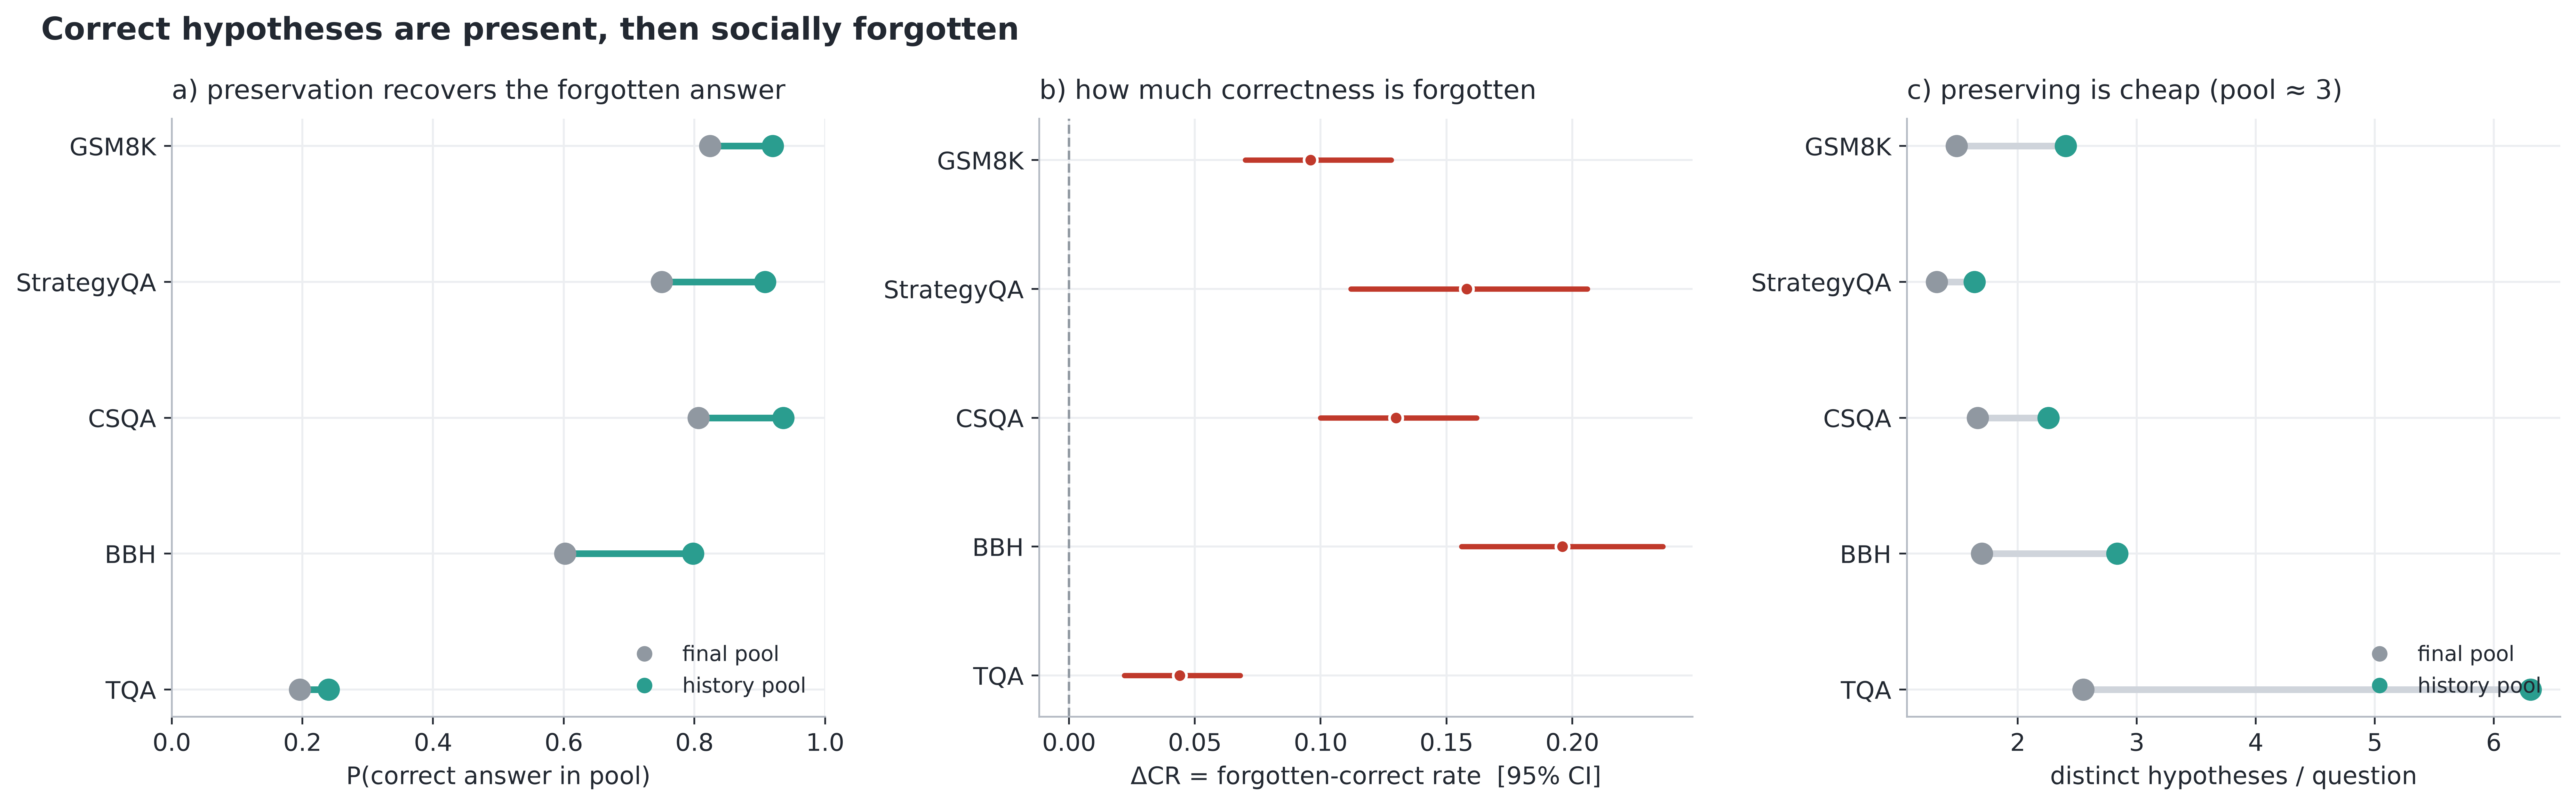
\includegraphics[width=\linewidth]{results/figures/fig2_extinction.png}
\caption{\textbf{Correct hypotheses are generated, then forgotten.} Per benchmark, the correct answer is
present in the history far more often than in the final round; the gap ($\Delta\mathrm{CR}$) is the
extinction rate, significant everywhere and largest on BBH.}
\label{fig:extinction}
\end{figure}

\paragraph{Anatomy of extinction.}
\label{par:extinction_anatomy}
The loss has a reproducible anatomy (Appendix~\ref{app:anatomy}). Two behavioral mechanisms drive it:
\emph{social adoption} (an agent copies a peer's wrong answer) and \emph{self-error drift} (an agent
revises its own correct answer away). Social adoption dominates overall ($\approx 72\%$ of extinctions),
but on the open-answer GSM8K anchor the loss is self-error-led ($57\%$ vs $43\%$). Notably, $73\%$ of
adoptions are \emph{surface}: the answer copies a peer while the reasoning does \emph{not} converge --- a
fact we return to in \S\ref{par:genuine_surface}. A lone correct minority is extinguished $78\%$ of the
time.

\paragraph{Information retained in the debate history.}
\label{par:history_information}
Preserving the full history is thus not a matter of adding noise: the history pool contains only
$\approx 3$ distinct hypotheses per question (Table~\ref{tab:preserve}, last column), yet recovering it
raises candidate recall from $0.636$ to $0.760$. An independent behavioral accounting agrees: censoring
truncation artifacts, $+11.6$pp of pooled accuracy is \emph{online-recoverable} --- present at some round
but discarded by the final vote --- rising to $+15.8$pp on BBH (Appendix~\ref{app:anatomy}).

\paragraph{Preservation headroom.}
\label{par:preservation_headroom}
Taken together, the total gap between the deployed majority ($50.9\%$) and a perfect selector over the
preserved pool ($76.0\%$) is $+25$ points, decomposing into $+12.5$pp of structural preservation and
$+12.7$pp of final-round selection. This headroom --- large, cheap, and present without any targeting --- is
the opportunity the rest of the paper pursues.


\subsection{Why Agent Influence Is Not Enough}
\label{subsec:influence_insufficient}

If debate forgets correct answers because some agents pull the group the wrong way, the natural remedy is
to identify influential agents and weight the vote by influence. This was the premise of our conference
work; here we show it is insufficient, which motivates the shift from agents to hypotheses. The full
influence analysis is in Appendix~\ref{app:influence}.

\paragraph{Influence structure in multi-agent debate.}
\label{par:influence_structure}
Influence, estimated as a PageRank centrality over an agent-to-agent adoption graph
(Appendix~\ref{app:influence}), is concentrated, stable across tasks (mean pairwise rank correlation
$0.80$), and persona-driven. But it is earned by \emph{stubbornness}, not correctness: across (agent,
benchmark) pairs, influence correlates with an agent's refusal to change ($r=0.69$, $p=0.005$) and not with
its standalone accuracy ($r=0.15$, $p=0.60$).

\paragraph{Influence and extinction mechanism.}
\label{par:influence_extinction}
Because influence tracks stubbornness, it cannot tell whether a given revision was a helpful correction or
a harmful capitulation. Predicting the extinction \emph{mechanism} (social adoption vs.\ self-error) from
influence features is at chance (AUC $0.49$; permutation floor $0.51$), whereas simple structural features
of the disagreement reach AUC $0.63$ --- influence describes \emph{how} opinions move but not
\emph{whether} the moved-to hypothesis is right.

\paragraph{Limits of influence-aware aggregation.}
\label{par:influence_aggregation}
Consequently, an influence-weighted vote does not help. Applied uniformly it \emph{loses} to plain
majority ($0.502$ vs.\ $0.528$ pooled; $\Delta=-0.026$, CI $[-0.036,-0.018]$), significantly so on GSM8K,
BBH, and CommonsenseQA (Table~\ref{tab:selector}). The relevant unit of analysis is therefore not the
agent that leads the debate but the evidential history of the hypothesis being selected --- the pivot to
provenance.


\subsection{The Gap Between Failure Prediction and Actionability}
\label{subsec:prediction_actionability}

The second natural remedy is to detect a failing debate and intervene. We show the detection half is
easy and the targeting half is not, which is why we ultimately abandon targeting altogether. The full
battery, summarized in Figure~\ref{fig:benefit} (Appendix~\ref{app:benefit}), is reported in
Appendix~\ref{app:benefit}.

\paragraph{Predicting impending extinction.}
\label{par:extinction_prediction}
A round-$0$ hazard detector predicts which debates will lose their correct answer with ROC $0.757$
in-distribution ($0.67$--$0.75$ leave-one-benchmark-out); extinction is genuinely detectable, most
strongly on StrategyQA (hazard ROC $0.87$). A mechanism-agnostic re-query can rescue a failing debate,
lifting preservation by $+16$pp at matched call count (Appendix~\ref{app:benefit}).

\paragraph{Oracle intervention headroom.}
\label{par:oracle_headroom}
Because our precompute stored both counterfactual arms for every debate, we observe the individual
treatment effect $\mathrm{ITE}_i=Y_1^{(i)}-Y_0^{(i)}$ of intervening. An \emph{oracle} that targets the
true ITE reaches always-on accuracy at a $\sim\!20\%$ budget, a gain of $+16.5$pp pooled ($+11.8$ on
GSM8K, $+20.4$ on BBH) --- the payoff from correct targeting is large and real.

\paragraph{Predicting individual intervention benefit.}
\label{par:benefit_prediction}
Yet none of that headroom is reachable from the pre-intervention state. The control outcome $Y_0$ is
predictable (OOF AUC $0.73$ --- essentially the hazard) and $Y_1$ is predictable (AUC $0.67$), but their
\emph{difference} is not: predicting whether intervention has any effect is barely above chance (AUC
$0.58$) and predicting its sign fails outright (learned CATE anti-correlated with true ITE). Five
pre-registered attempts with progressively richer signals --- cheap structural features, residualized
semantic embeddings, an active self-diagnosis probe, a placebo-controlled dose-response probe, and the
mid-debate trajectory --- all fail the same benefit gate (Appendix~\ref{app:benefit}).

\paragraph{Predictability does not imply actionability.}
\label{par:predictability_actionability}
The lesson is a clean impossibility for our setting: \emph{failure prediction and benefit prediction are
different problems, and only the first is solved from the observable state.} Differencing two individually
predictable outcomes leaves a treatment effect the transcript does not determine. A hazard-guided
controller therefore matches always-on intervention at $\sim\!55\%$ fewer interventions but cannot beat a
random budget (its one significant effect is a rescue-$\gg$-harm asymmetry; Appendix~\ref{app:controller}).
Rather than keep searching for a controller, we address the loss structurally.


\subsection{Provenance as a Signal of Hypothesis Correctness}
\label{subsec:provenance_correctness}

Having preserved the hypotheses (\S\ref{subsec:extinction_results}), we ask whether a hypothesis's own
provenance --- computed with no new LLM calls --- tells us if it is correct. It does, on every one of the
eight benchmarks (Table~\ref{tab:prov}, Figure~\ref{fig:provbench}).

\paragraph{Candidate-level provenance signal.}
\label{par:candidate_signal}
At the candidate level (base rate $\Pr(\text{correct})=0.25$), independent support, persistence, and first
round of appearance each predict correctness monotonically and across benchmarks. The distinction is
stark: an answer produced independently by three agents is $83\%$ correct, whereas one that only
\emph{emerges} during the debate is $\approx 7\%$ correct --- a difference the majority vote discards
entirely.

\begin{table}[t]
\centering\small
\caption{Provenance predicts correctness (candidate level; directional AUC with clustered-boot CI, and
$\Pr(\text{correct})$ by feature value). Independent support and persistence are monotone across
benchmarks; late-adoption and ``resurrected'' features are near chance (honesty controls).}
\label{tab:prov}
\begin{tabular}{lccl}
\toprule
Signal & dir.\ AUC [95\% CI] & mono. & $\Pr(\text{correct}\mid\cdot)$ \\
\midrule
$n_{\mathrm{ind}}$ (round-0 support) & $0.823\,[.800,.845]$ & 4/5 & $0{:}.07\;\;1{:}.17\;\;2{:}.58\;\;3{:}.83$ \\
$n_{\mathrm{per}}$ (rounds alive)    & $0.806\,[.785,.824]$ & 5/5 & $1{:}.06\;\;2{:}.30\;\;3{:}.57$ \\
$n_{\mathrm{sup}}$ (total votes)     & $0.857\,[.836,.877]$ & 2/5 & $.05\!\rightarrow\!.84$ \\
first round (late emergence)         & $0.695\,[.681,.709]$ & 4/5 & $r_0{:}.37\;\;r_1{:}.08\;\;r_2{:}.04$ \\
\bottomrule
\end{tabular}
\end{table}

\begin{figure}[t]
\centering
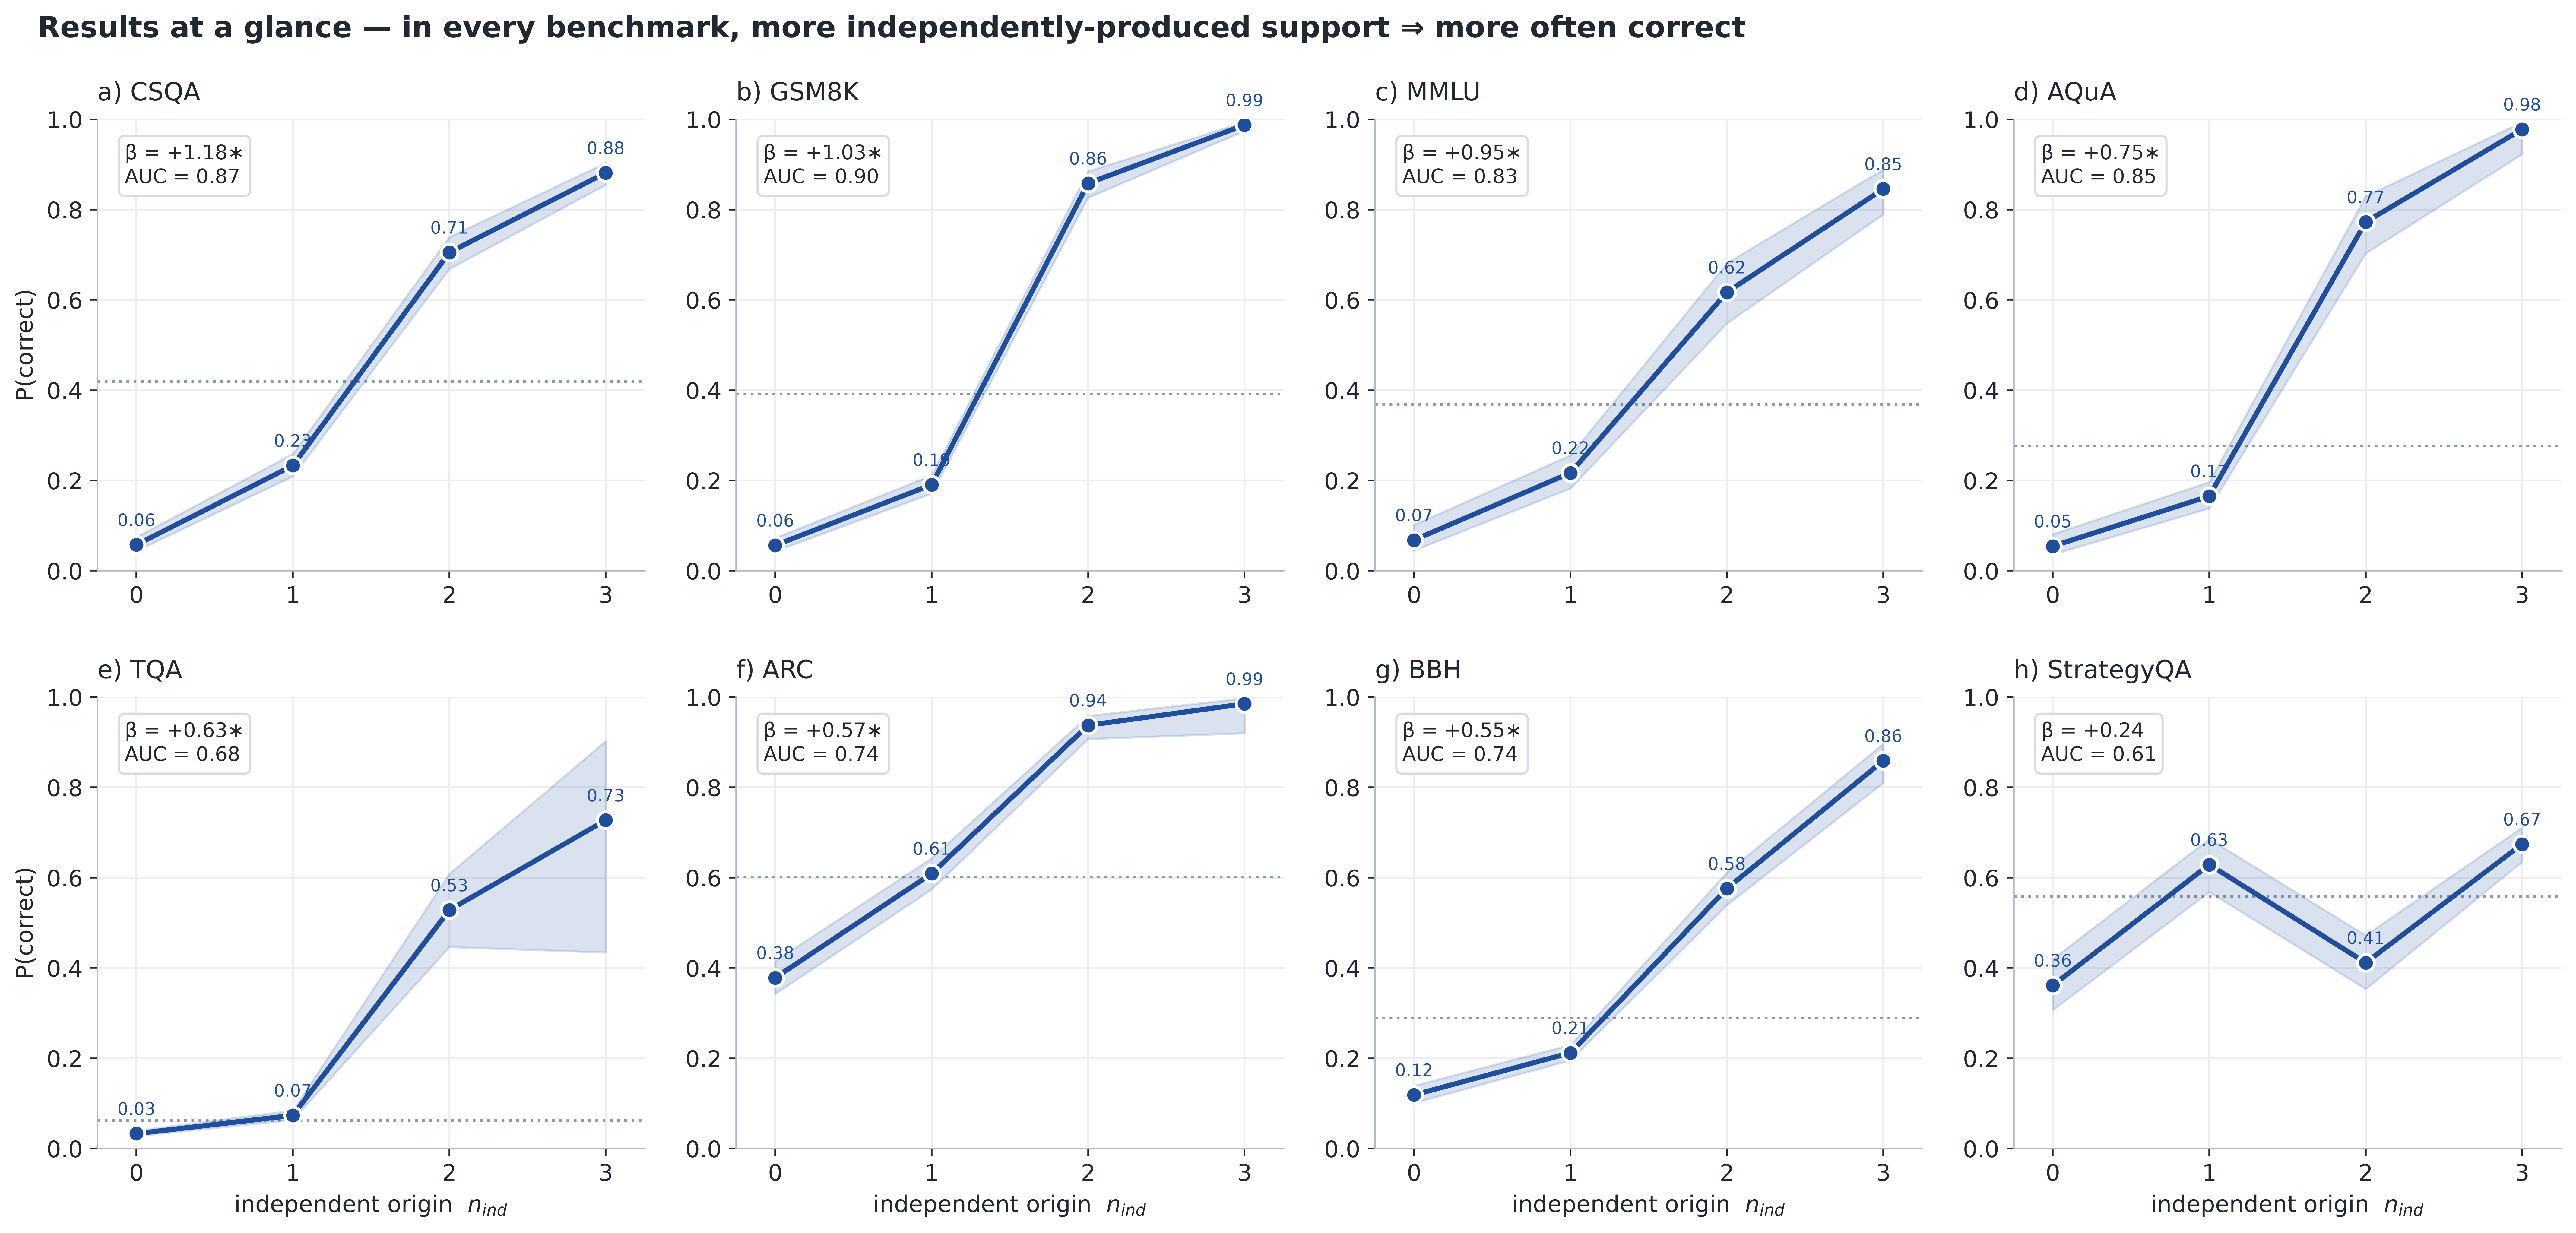
\includegraphics[width=\linewidth]{results/figures/fig10_overview.png}
\caption{\textbf{Provenance predicts correctness, at a glance, on every benchmark.} Per benchmark,
$\Pr(\text{correct})$ rises with the number of independently produced supporters ($n_{\mathrm{ind}}$): more
independent origins means more often correct, across all eight tasks. Per-feature reliability curves and
feature-importance rankings are in Figure~\ref{fig:reliability} and Figure~\ref{fig:features}
(Appendix~\ref{app:e26}).}
\label{fig:provbench}
\end{figure}

\paragraph{Independent origins.}
\label{par:independent_correctness}
Independent support is the strongest single origin signal, with directional AUC $0.823$ and correctness
climbing $0.07\!\to\!0.17\!\to\!0.58\!\to\!0.83$ as $n_{\mathrm{ind}}$ rises from $0$ to $3$. This is the
quantity we sharpen in \S\ref{subsec:not_all_consensus_equal}.

\paragraph{Persistence and temporal history.}
\label{par:persistence_correctness}
Persistence is a second, weaker dimension (AUC $0.806$, monotone on all five benchmarks): hypotheses that
survive more rounds are more likely correct. Conversely, the first round of appearance is a strong
negative signal --- answers that appear only after round $0$ are correct just $8\%$ (round 1) and $4\%$
(round 2) of the time, versus $37\%$ at round $0$, quantifying the destructiveness of debate revision.

\paragraph{Comparative informativeness of provenance features.}
\label{par:provenance_comparison}
Total support has the highest raw AUC ($0.857$) but a noisy, non-monotone tail (monotone on only $2/5$
benchmarks), and an equal-weight combination of provenance features reaches AUC $0.827$ (per-feature AUCs
in Figure~\ref{fig:features}, Appendix~\ref{app:e26}). This sets up the
central question: total support and independent support are strongly correlated, so \emph{is it the
magnitude of agreement that matters, or its origin?} The next subsection answers it.


\subsection{Not All Consensus Is Equally Informative}
\label{subsec:not_all_consensus_equal}

This is the paper's central finding. Consensus is not a homogeneous count of votes: at \emph{matched total
support}, independently generated agreement carries substantially more correctness signal than socially
inherited agreement (Figure~\ref{fig:matched}). The analysis spans $23{,}239$ candidates over five
ensembles and eight benchmarks, with clustered bootstraps over (config, benchmark, question).

\paragraph{Correctness under matched total support.}
\label{par:matched_support_results}
Fixing total support and varying only how it was formed makes the effect visible without any model
(Table~\ref{tab:matched}). Among hypotheses with total support $n_{\mathrm{sup}}=4$, correctness rises
from $0.21$ when none of the support is independently generated to $0.44$, $0.66$, and $0.74$ as the number
of independent origins goes from one to three. The same upward slope holds at every support level for which
the strata are populated --- the hallmark of a signal that magnitude alone cannot explain.

\begin{table}[t]
\centering\small
\caption{Correctness at \emph{matched total support}. Each row fixes total support $n_{\mathrm{sup}}$; each
column varies the number of independent (round-0) origins $n_{\mathrm{ind}}$. Within every row, more
independent origins means higher correctness, though total support is identical. Cells show
$\Pr(\text{correct})$ (candidate count).}
\label{tab:matched}
\begin{tabular}{lcccc}
\toprule
$n_{\mathrm{sup}}$ & $n_{\mathrm{ind}}{=}0$ & $n_{\mathrm{ind}}{=}1$ & $n_{\mathrm{ind}}{=}2$ & $n_{\mathrm{ind}}{=}3$ \\
\midrule
2 & $0.13\,(1383)$ & $0.20\,(1610)$ & $0.38\,(196)$  & --- \\
3 & $0.19\,(382)$  & $0.31\,(1554)$ & $0.52\,(276)$  & --- \\
4 & $0.21\,(156)$  & $0.44\,(739)$  & $0.66\,(458)$  & $0.74\,(43)$ \\
5 & $0.28\,(47)$   & $0.48\,(545)$  & $0.71\,(666)$  & $0.80\,(95)$ \\
6 & ---            & $0.53\,(231)$  & $0.78\,(652)$  & $0.87\,(534)$ \\
\bottomrule
\end{tabular}
\end{table}

\begin{figure}[t]
\centering
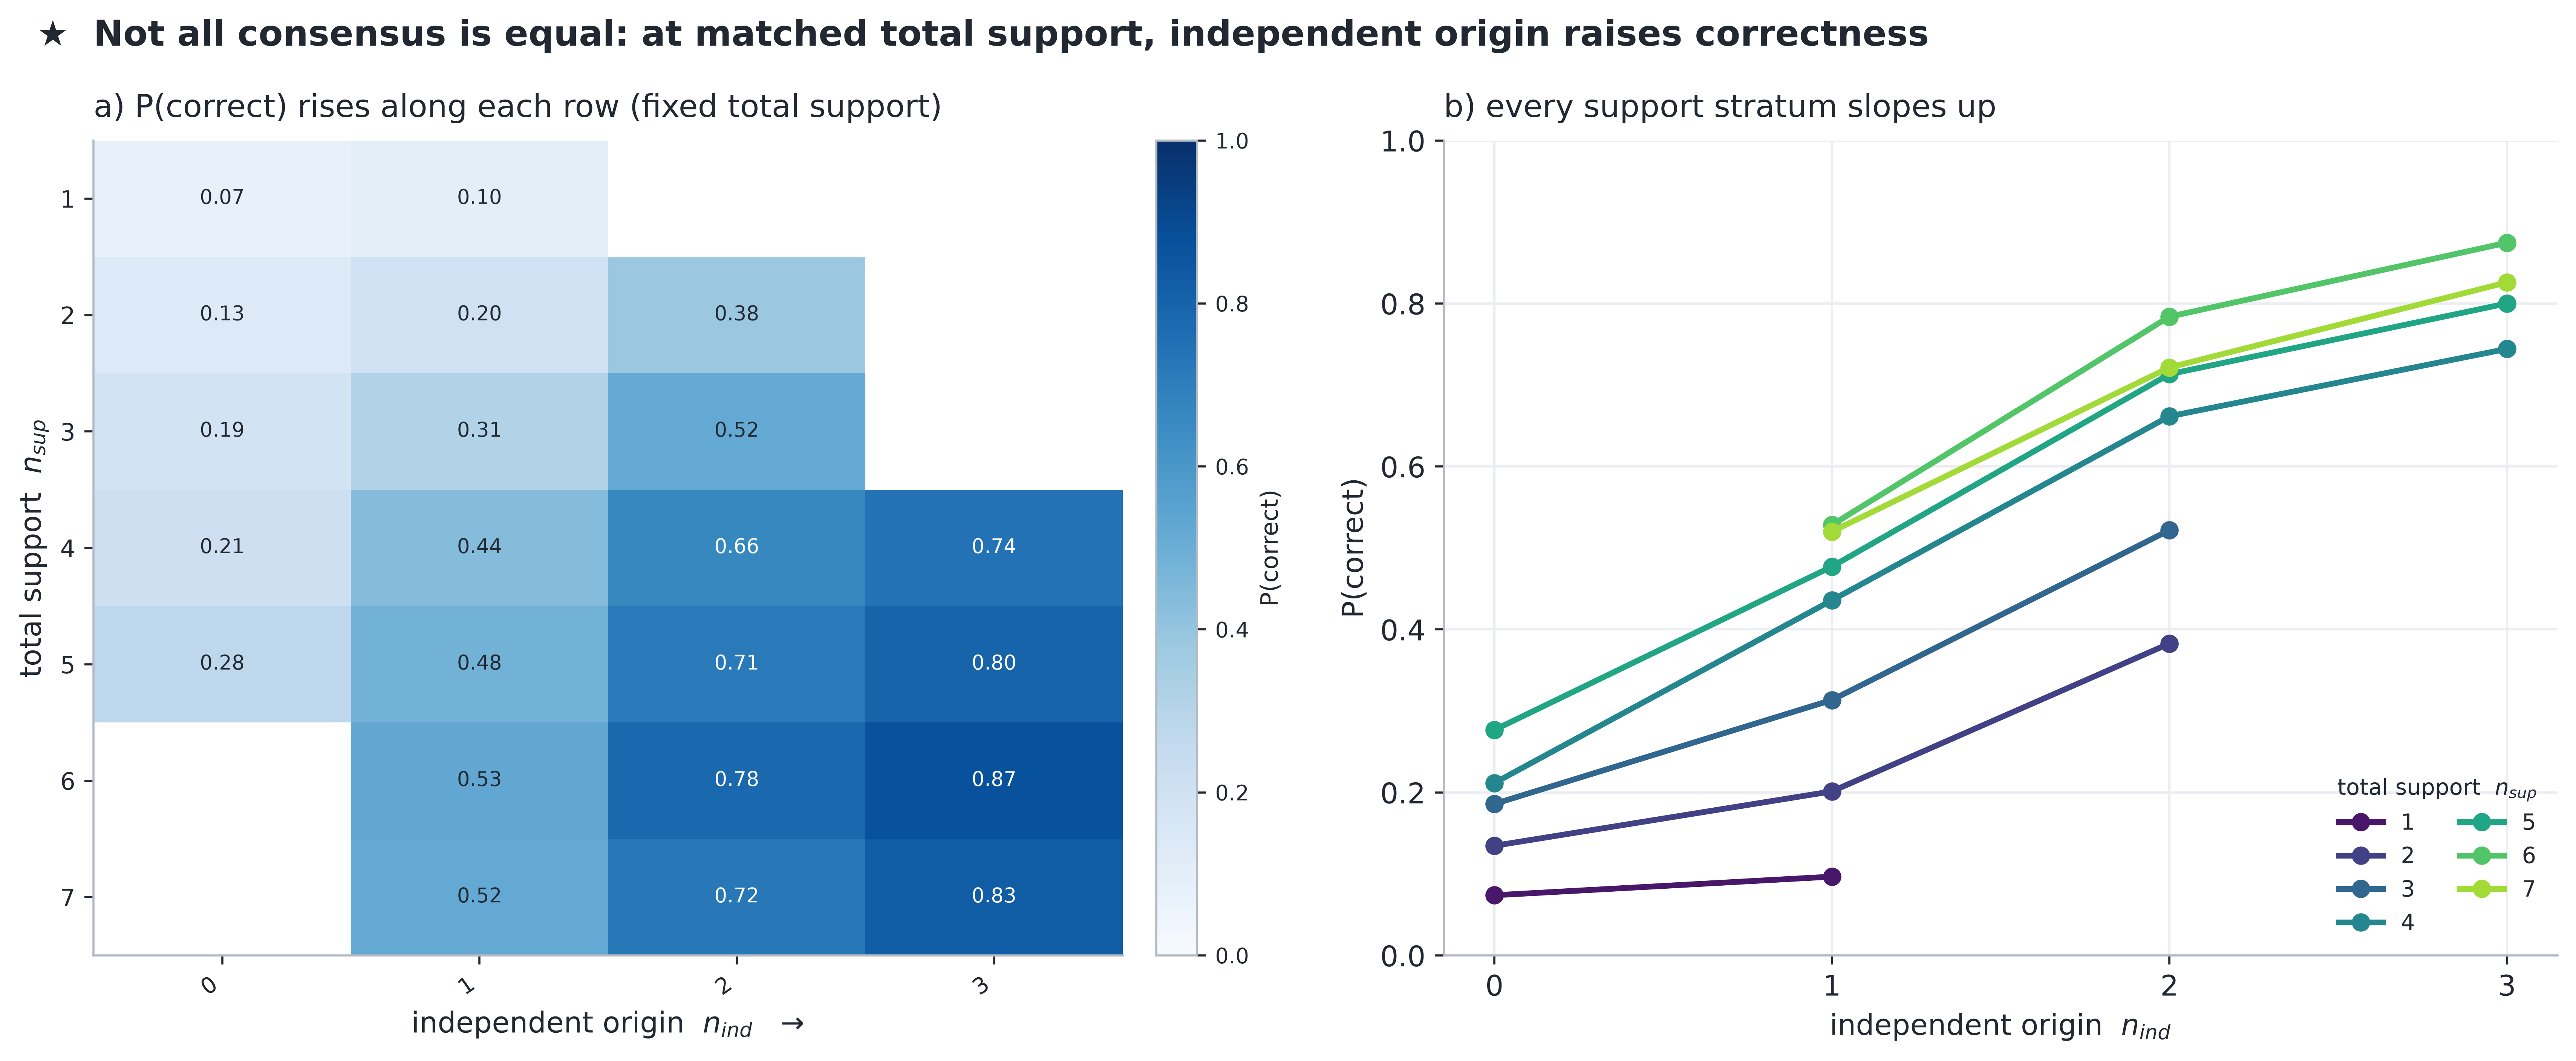
\includegraphics[width=\linewidth]{results/figures/fig5_matched_support_HERO.png}
\caption{\textbf{Not all consensus is equal (H3, hero).} Two candidates with identical total support can
carry very different reliability: $\Pr(\text{correct})$ increases with the number of independent origins
\emph{within} each fixed-total-support stratum. Origin, not magnitude, is what tracks correctness.}
\label{fig:matched}
\end{figure}

\paragraph{Independent versus socially inherited agreement.}
\label{par:independent_inherited_results}
Parametrically, decomposing support into its independent and inherited components gives per-vote log-odds
of $\beta_{\mathrm{ind}}=1.035$ ($[0.963,1.112]$) versus $\beta_{\mathrm{inh}}=0.386$ ($[0.354,0.420]$) ---
an independently generated vote is worth about $2.68\times$ an inherited one
(Table~\ref{tab:coef}, Figure~\ref{fig:coef}). Equivalently, controlling for total support, each additional
independent origin adds $\beta_{\mathrm{ind}}=0.649$ ($[0.565,0.737]$) to the log-odds of correctness. We
interpret this as an \emph{epistemic signal}: origin is associated with correctness after conditioning on
consensus magnitude; the observational logs do not license a causal claim that manufacturing independent
support would make an answer correct.

\begin{table}[t]
\centering\small
\caption{Origin carries correctness signal beyond magnitude ($n{=}23{,}239$ candidates; clustered-boot
$95\%$ CIs). Model~A controls total support; Model~B decomposes support per vote; both agree that
independent support dominates inherited support. Effects survive benchmark$+$config fixed effects and a
joint model with persistence.}
\label{tab:coef}
\begin{tabular}{llc}
\toprule
Model & Coefficient & Estimate [95\% CI] \\
\midrule
A: control $n_{\mathrm{sup}}$        & $\beta_{\mathrm{ind}}$ (per independent origin) & $0.649\,[0.565,0.737]$ \\
B: decomposition                     & $\beta_{\mathrm{ind}}$ (per independent vote)   & $1.035\,[0.963,1.112]$ \\
                                     & $\beta_{\mathrm{inh}}$ (per inherited vote)     & $0.386\,[0.354,0.420]$ \\
A $+$ bench\,\&\,config FE           & $\beta_{\mathrm{ind}}$                          & $0.656\,[0.577,0.748]$ \\
Joint $\{$ind, inh, persist$\}$      & $\beta_{\mathrm{ind}}$                          & $0.950\,[0.877,1.028]$ \\
                                     & $\beta_{\mathrm{inh}}$                          & $0.228\,[0.188,0.271]$ \\
                                     & $\beta_{\mathrm{per}}$                          & $0.448\,[0.367,0.524]$ \\
\bottomrule
\end{tabular}
\end{table}

\begin{figure}[t]
\centering
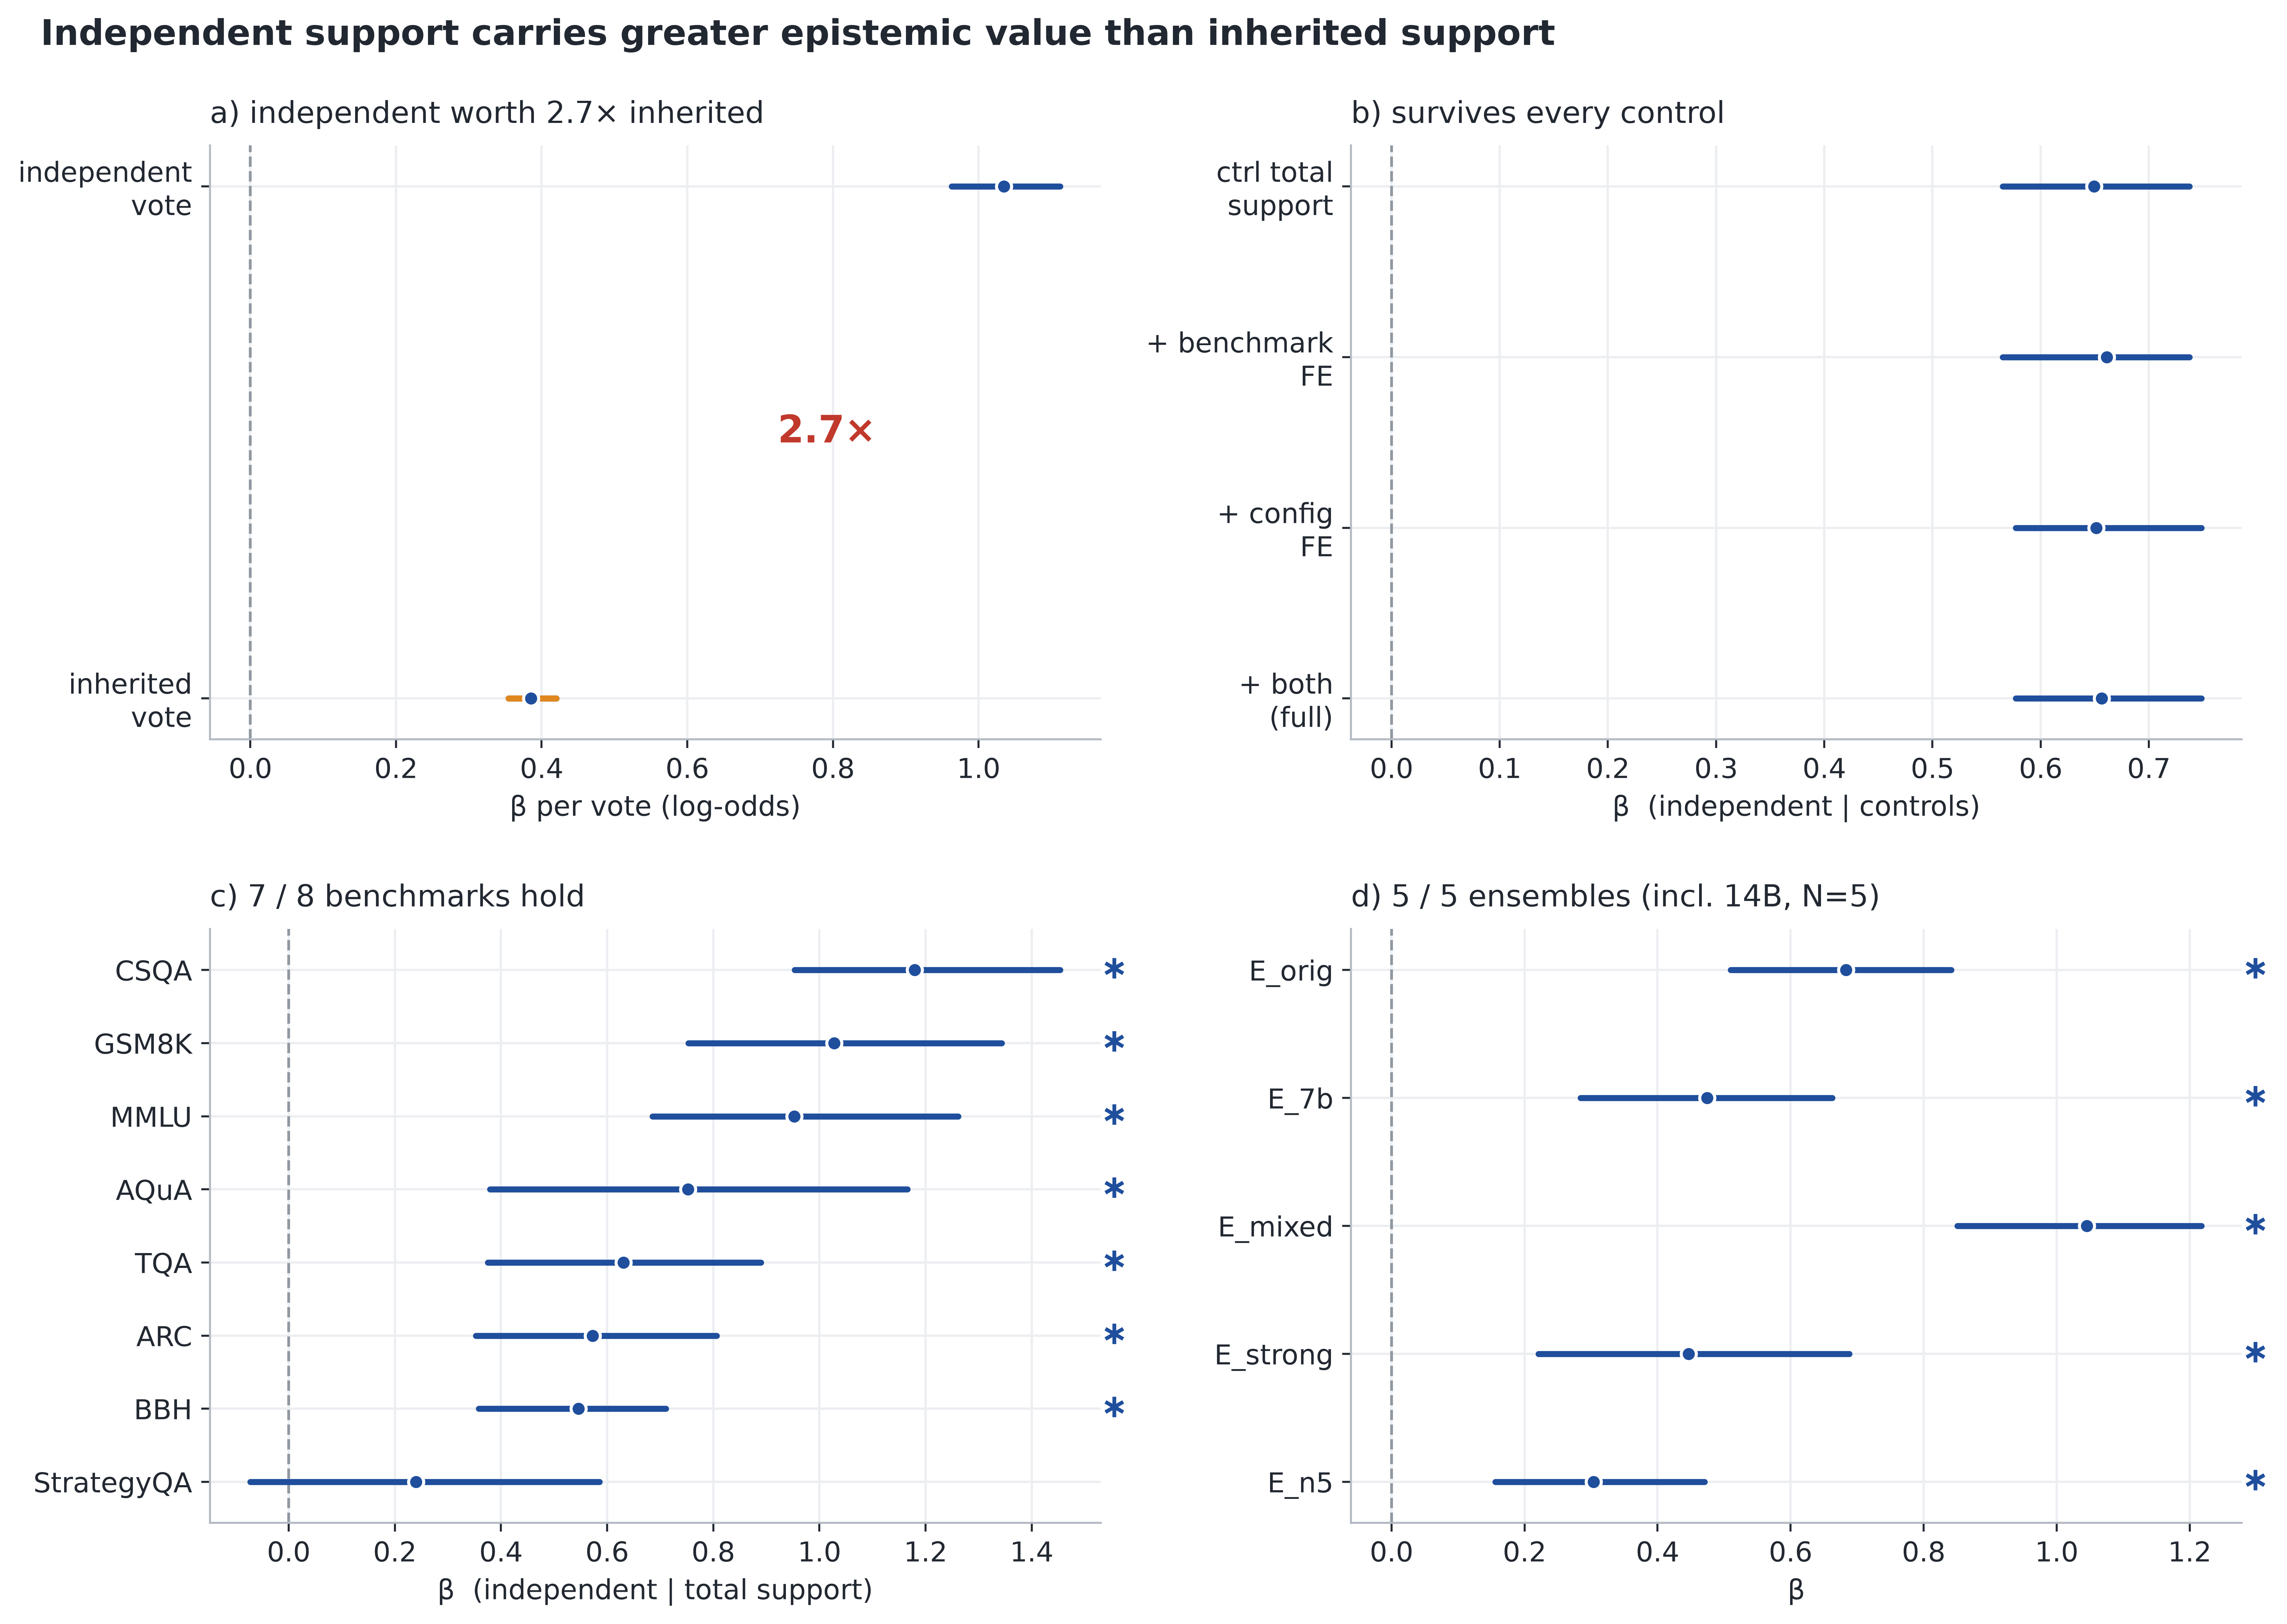
\includegraphics[width=\linewidth]{results/figures/fig6_coefficients.png}
\caption{\textbf{The origin effect is not a proxy for magnitude.} The partial coefficient on independent
support stays well clear of zero as we add controls (total support, benchmark and config fixed effects, and
persistence), and per vote it far exceeds inherited support ($\approx 2.7\times$).}
\label{fig:coef}
\end{figure}

\paragraph{Controlling for benchmark and ensemble effects.}
\label{par:fixed_effect_results}
The effect is not an artifact of task or ensemble mix. Adding benchmark and configuration fixed effects
leaves it essentially unchanged ($\beta_{\mathrm{ind}}=0.656$, $[0.577,0.748]$), and a joint model that
includes persistence keeps all three provenance dimensions clear of zero, with the ordering
independent $>$ persistence $>$ inherited (Table~\ref{tab:coef}).

\paragraph{Consistency across benchmarks.}
\label{par:h3_benchmarks}
Per benchmark, the partial independent-support effect is positive and significant on seven of the eight
benchmarks (GSM8K, CommonsenseQA, BBH, TruthfulQA, AQuA, MMLU, ARC; full estimates in
Table~\ref{tab:e26_bench}, Appendix~\ref{app:e26}). StrategyQA is the lone boundary case
($\beta_{\mathrm{ind}}=0.240$, $[-0.072,0.586]$, CI includes zero) --- its binary answer space affords
little room for multiple independent origins to differentiate, consistent with StrategyQA being the one
benchmark on which debate is net-constructive.

\paragraph{Consistency across model and agent configurations.}
\label{par:h3_configs}
Per configuration, the effect holds on all five ensembles, including the strong-anchor ensemble with a
$14$B model ($\beta_{\mathrm{ind}}=0.447$, $[0.221,0.688]$) and the five-agent ensemble
($\beta_{\mathrm{ind}}=0.304$, $[0.156,0.471]$). The principle is therefore not tied to weak $3$B debaters
or to $N=3$; the full per-benchmark table (Table~\ref{tab:e26_bench}) and per-config estimates are in
Appendix~\ref{app:e26}.

\paragraph{Epistemic mechanism versus incremental prediction.}
\label{par:mechanism_prediction}
One caveat is essential and, in fact, sets up the next subsection. Because independent and total support
are collinear ($r=0.83$), adding independent support \emph{on top of} total support raises candidate-level
ranking AUC by only $+0.007$ ($0.841\!\to\!0.849$). H3 is thus a statement about epistemic value
\emph{per vote}, not about incremental ranking power --- and this small increment is precisely why the
downstream selector, which can only exploit ranking information, delivers a real but modest and
regime-bound gain.


\subsection{From Epistemic Mechanism to Decision Utility}
\label{subsec:decision_utility}

We now convert the mechanism into a decision rule. We treat provenance-aware selection as a
\emph{downstream application} of the central finding, not the paper's headline: it recovers part of the
preservation headroom at zero additional cost, but its accuracy gain is conditional
(Table~\ref{tab:selector}; see also the selector ladder in Figure~\ref{fig:ladder} and the applicability
landscape in Figure~\ref{fig:utility}, Appendix~\ref{app:selectors}).

\paragraph{Provenance-aware re-selection.}
\label{par:selector_results}
The frozen provenance selector (\S\ref{subsec:provenance_selection}), scoring each preserved hypothesis by
its independent support, persistence, total support, and recency, improves pooled accuracy from the deployed
majority's $0.528$ to $0.564$ ($\Delta=+0.035$, CI $[+0.022,+0.049]$; up to $+8$pp on some benchmarks) with
\textbf{no additional inference}. Equal-weight and cross-fit logistic variants agree.

\begin{table}[t]
\centering\small
\caption{Inference-time selection rules over the frozen debate logs (gold-free; clustered-boot CI over
questions). Provenance beats the deployed majority and the conference influence vote at zero extra LLM
calls; influence voting and an external judge lose. Oracle $=$ a perfect selector over the preserved pool.}
\label{tab:selector}
\begin{tabular}{lccc}
\toprule
Selector & Pooled acc & $\Delta$ vs.\ majority [95\% CI] & Extra calls \\
\midrule
Final majority (deployed)           & 0.528 & --- & 0 \\
Conference influence voting         & 0.502 & $-0.026\,[-.036,-.018]$ & 0 \\
Round-0 (independent) majority      & 0.560 & $+0.032\,[.015,.048]$ & 0 \\
\textbf{Provenance selector (ours)} & \textbf{0.564} & $\mathbf{+0.035\,[.022,.049]}$ & \textbf{0} \\
\midrule
Oracle (history-pool ceiling)       & 0.760 & $+0.232$ & --- \\
\bottomrule
\end{tabular}
\end{table}

\paragraph{Comparison with consensus and influence-based aggregation.}
\label{par:selector_comparison}
The selector beats the deployed final majority and, more pointedly, beats the conference influence vote,
which itself \emph{loses} to plain majority (\S\ref{par:influence_aggregation}) --- provenance succeeds
exactly where influence weighting fails. An external LLM judge is worse still: forced to pick from the
preserved pool, both a $7$B and a $14$B judge fail the preservation gate
($\Delta_{\mathrm{HP}}=-0.047$ and $-0.018$), and the $14$B model scores higher \emph{solving} the question
($0.76$) than \emph{selecting} from a weak pool ($0.53$) --- a capable external judge is a liability under
capability mismatch, not a fix (Appendix~\ref{app:selectors}).

\paragraph{The independent-majority baseline.}
\label{par:independent_majority}
The provenance selector ties a strikingly simple baseline: taking the round-$0$ independent majority
($0.560$). This is not a weakness of the method but a restatement of the phenomenon --- trusting the
pre-debate answer is strong precisely because debate is net-destructive on four of five benchmarks
(\S\ref{subsec:extinction_results}). What wins is independent agreement, whether read as a vote or as a
provenance feature; the sophistication of the score is not what matters.

\paragraph{Recoverable headroom and realized gain.}
\label{par:realized_gain}
The selector captures roughly $14$--$15\%$ of the $+23$pp preservation ceiling. The remaining $\approx 86\%$
requires a selector that can verify a candidate's reasoning, not merely rank its provenance --- our stated
open problem.

\paragraph{Why the downstream gain is necessarily modest.}
\label{par:modest_gain}
The ceiling on the gain is exactly the $+0.007$ incremental AUC of \S\ref{par:mechanism_prediction}: origin
carries large per-vote epistemic value, but because it co-varies with total support, a rank-based selector
that already uses support cannot extract much more. The strong mechanism and the modest selector are two
faces of the same collinearity, not a contradiction.

\paragraph{Applicability across debate regimes.}
\label{par:applicability}
Consistent with this, the accuracy gain is regime-bound: significant in $15$ of $40$ generalization cells,
with \emph{no} cell showing a significant loss (every failing CI includes zero). It is a conditional
improvement, not a universal one.

\paragraph{Identifiability and candidate availability.}
\label{par:identifiability_availability}
Two conditions govern when the selector helps: provenance must be \emph{informative} about correctness
(identifiability) and a correct hypothesis must be \emph{available} in the preserved pool (availability).
Both hold on multi-answer reasoning benchmarks; StrategyQA violates identifiability (binary answers, and
the one net-constructive regime) and TruthfulQA violates availability (an adversarial, low-accuracy pool).
The applicability landscape --- gain against headroom and against identifiability --- is shown in
Figure~\ref{fig:utility} (Appendix~\ref{app:selectors}).


\subsection{Generalization Across Tasks and Debate Configurations}
\label{subsec:generalization}

To ensure the scientific claims are not artifacts of one setting, we re-ran the frozen analysis over a
grid of $40$ (configuration, benchmark) cells spanning five model families, capabilities from $3$B to
$14$B, agent populations $N\in\{3,5\}$, and eight benchmarks (Figure~\ref{fig:generalization}).

\paragraph{Across benchmark families.}
\label{par:generalization_benchmarks}
Extinction and the provenance signal appear on every benchmark family we tested --- arithmetic, binary
strategic, multiple-choice commonsense, mixed hard tasks, adversarial factuality, and the three added
multiple-choice sets (AQuA, MMLU, ARC).

\paragraph{Across model families and capability levels.}
\label{par:generalization_models}
Scaling the anchor from $3$B to $14$B raises majority accuracy while shrinking the remaining headroom, but
does not eliminate the phenomena: extinction and provenance$\to$correctness hold under the $14$B ensemble,
and the origin effect (H3) holds there too (\S\ref{par:h3_configs}).

\paragraph{Across agent populations.}
\label{par:generalization_agents}
Moving from $N=3$ to $N=5$ preserves all three hypotheses and, if anything, gives the selector slightly
more room (more independent origins to distinguish).

\paragraph{Generalization of the three central hypotheses.}
\label{par:generalization_hypotheses}
Quantitatively: \textbf{H1} (extinction) is directionally positive in all $40/40$ cells and strictly
significant in $35/40$ (the five near-misses are near-ceiling); \textbf{H2}
(provenance$\to$correctness) holds in $39/40$ (the sole exception being \textsc{E\_7b} on StrategyQA); and
\textbf{H3} (independent $>$ inherited at matched support) holds on $7/8$ benchmarks and $5/5$ ensembles.
The downstream \emph{selector} gain, by contrast, is significant in $15/40$ cells --- broad enough to be
useful, regime-bound as predicted. The two scientific claims travel; the utility is conditional
(Appendix~\ref{app:e26}).

\begin{figure}[t]
\centering
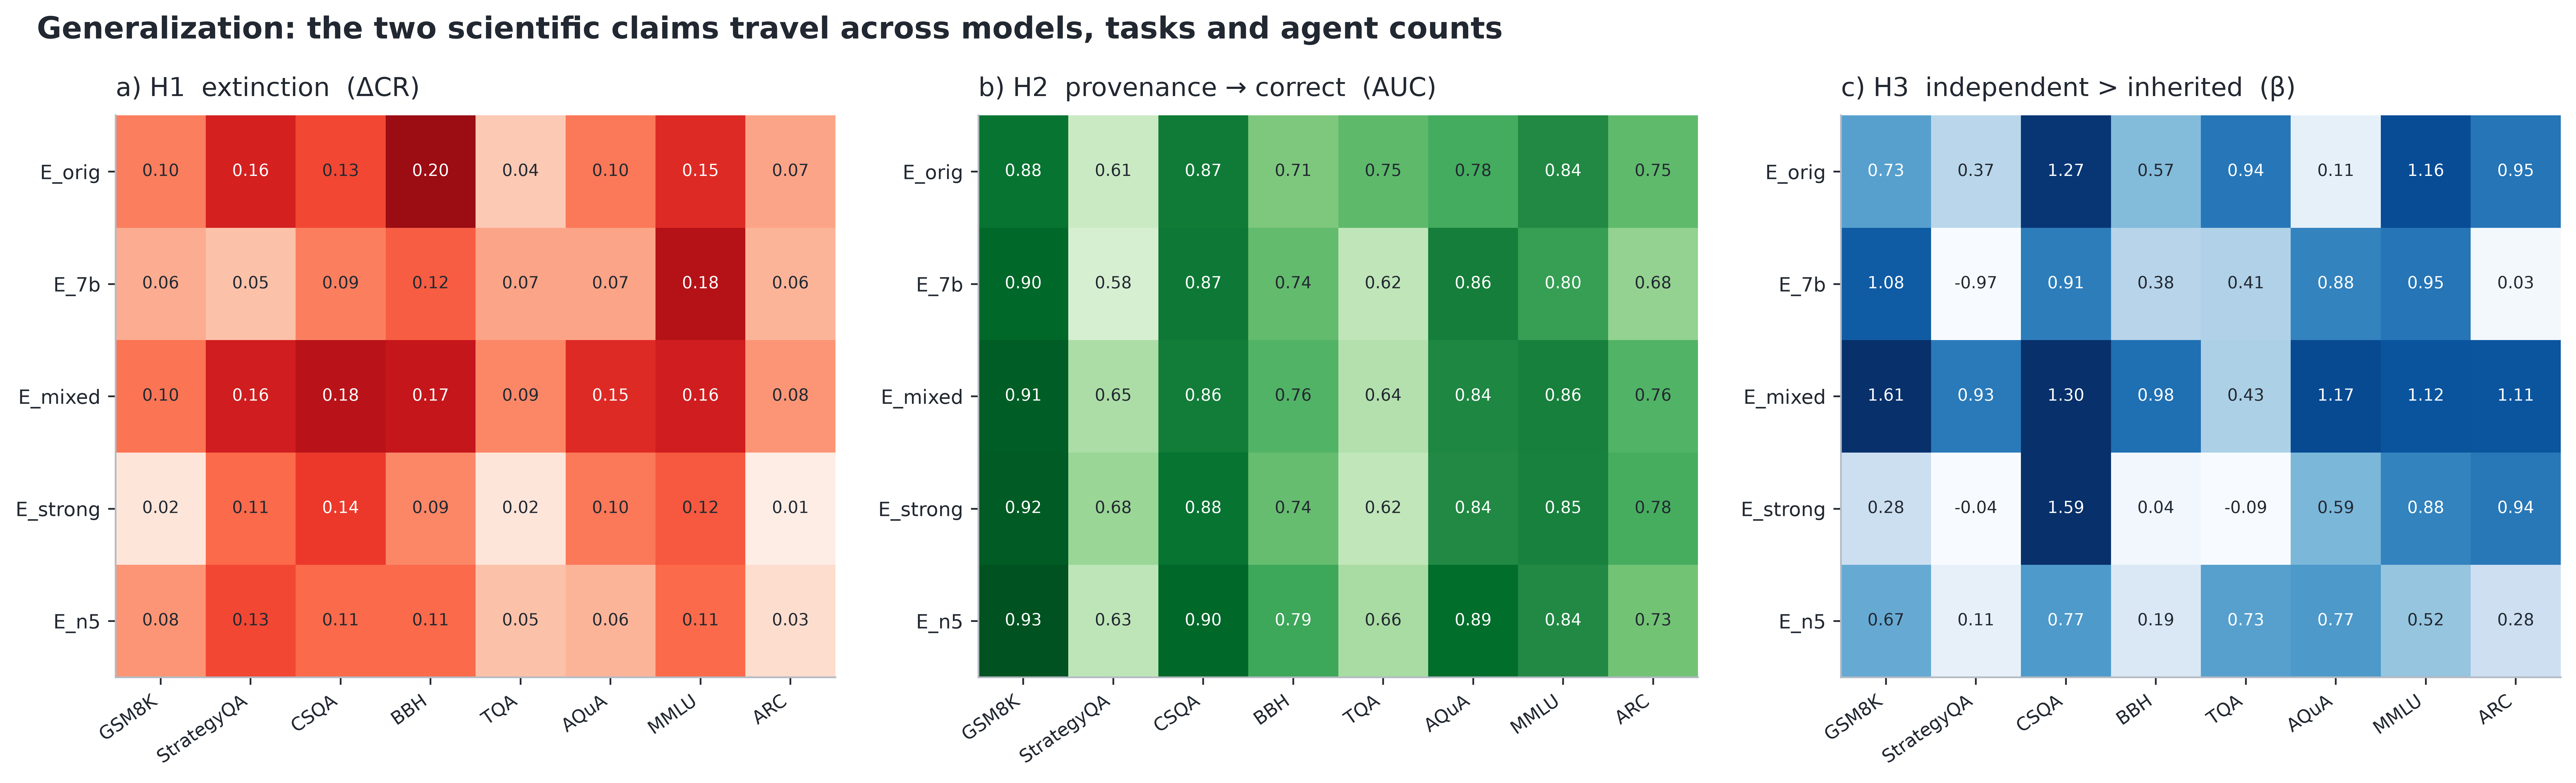
\includegraphics[width=\linewidth]{results/figures/fig7_generalization.png}
\caption{\textbf{Generalization atlas.} Across $40$ cells (5 ensembles $\times$ 8 benchmarks, $N\in\{3,5\}$,
$3$B--$14$B), extinction (H1) and provenance$\to$correctness (H2) are near-universal and the origin effect
(H3) holds on $7/8$ benchmarks and $5/5$ ensembles, while the selector's accuracy win stays regime-bound.}
\label{fig:generalization}
\end{figure}

\subsection{Additional Mechanistic Analyses}
\label{subsec:additional_analysis}

\paragraph{Genuine versus surface social adoption.}
\label{par:genuine_surface}
Does the origin effect merely reflect that some late adoptions genuinely converge in reasoning while others
copy at the surface? No: it is \emph{origin} that matters, not the quality of later adoption. A naive
event-level comparison suggests genuine adoptions are more correct than surface ones
($0.356$ vs.\ $0.292$, $\Delta=+0.064$), but once total support is controlled the genuine$-$surface
difference vanishes ($-0.014$, CI $[-0.111,+0.080]$), while independent support still towers over both
(Appendix~\ref{app:surface}). This is also a cautionary tale for the naive analysis --- exactly why H3
must be estimated at matched total support.

\paragraph{Independent origin versus reasoning convergence.}
\label{par:origin_convergence}
A convergence-gated selector, which credits late consensus only when supporters' reasoning genuinely
converges (lexical similarity residualized against the debate's own baseline), correctly recovers the one
constructive-debate benchmark (StrategyQA, $0.580\!\to\!0.604$) but cannot beat the round-$0$ majority
pooled: a single global rule cannot serve both the destructive and constructive regimes, and identifying
per-instance whether a revision is constructive is the mechanism-attribution problem that is at chance
(\S\ref{subsec:prediction_actionability}; Appendix~\ref{app:selectors}).

\paragraph{External LLM judging.}
\label{par:external_judge}
As noted in \S\ref{par:selector_comparison}, replacing the intrinsic provenance signal with an external LLM
judge fails: a capable judge does better solving the question than selecting from a weak debate pool
(Appendix~\ref{app:selectors}). This reinforces that the working signal is intrinsic to the debate's
provenance, not an added evaluator.

\paragraph{Boundary regimes and failure cases.}
\label{par:boundary_cases}
The honest boundaries are consistent across analyses: StrategyQA (binary, net-constructive debate) is where
H3 is not significant and the selector should not trust early answers, and TruthfulQA (adversarial, very
low base accuracy, noisy pool) is where availability fails. We report these as boundaries rather than hide
them; they delimit exactly where the method applies.


\section{Discussion}
\label{sec:discussion}

\subsection{Consensus as Epistemically Heterogeneous Evidence}
\label{subsec:epistemic_heterogeneity}
Our central result gives an LLM-specific operationalization of a classical principle: the reliability of
collective agreement depends on the dependence structure of the evidence producing it. Wisdom-of-crowds
reasoning is strongest when individual judgments are sufficiently independent, so that errors cancel rather
than reinforce; recent behavioral work shows that convergence among independent, approximately unbiased
informants rationally signals accuracy \cite{pfander2025crowd}. Multi-agent debate systematically violates
this assumption, because later-round votes are explicitly conditioned on peers. Rather than treat
independence as an unobserved assumption, we track it directly through provenance and show that, at matched
total support, independently generated agreement is worth about $2.7\times$ an inherited vote. Consensus, in
short, is epistemically heterogeneous: a vote count conflates \emph{how much} agreement exists with
\emph{how it was formed}.

\subsection{From Agent Influence to Hypothesis Provenance}
\label{subsec:influence_to_provenance}
This reframes an influence-centered view of debate (Figure~\ref{fig:interpretation},
Appendix~\ref{app:influence}). Influence describes
how opinions propagate --- who is followed, who holds their ground --- and centrality measures such as
PageRank quantify it well \cite{page1998pagerank,zhang2024collaboration}. But influence is silent on
correctness: a highly influential agent can propagate a right or a wrong hypothesis, and our data show
influence is earned by stubbornness, not accuracy, so an influence-weighted vote can underperform plain
majority. The unit that carries reliability is not the agent that leads the debate but the evidential
history of the hypothesis being selected. Shifting the question from ``who supplied this answer?'' to ``how
many independent paths produced it?'' is the conceptual move from influence to provenance.

\subsection{Why Mechanistic Signal Does Not Guarantee Decision Gain}
\label{subsec:mechanism_utility}
A recurring theme is that a strong mechanism need not yield a large decision improvement. Independent origin
carries substantial per-vote epistemic value, yet because it co-varies with total support ($r=0.83$), it
adds only $+0.007$ ranking AUC over raw consensus, and a rank-based selector therefore recovers only
$\approx 14\%$ of the preservation ceiling. This mirrors the failure-vs-benefit result: two quantities can
each be predictable while the decision-relevant contrast between them is not. Honest reliability engineering
must separate the size of a mechanism from its incremental decision utility --- and report both.

\subsection{Implications for Multi-Agent LLM Design}
\label{subsec:design_implications}
Three design implications follow. First, \emph{do not destructively overwrite hypotheses}: preserving the
history pool is nearly free (about three candidates per question) and exposes a large recoverable headroom.
Second, \emph{prefer independent corroboration to social consensus}: independently generated agreement is a
cheap, model-agnostic reliability signal, whereas agreement acquired after peer exposure --- and influence
weighting built on it --- should be discounted. Third, \emph{be wary of external judges under capability
mismatch}: a strong judge does better solving a problem than adjudicating a weak pool, so a matched-class,
intrinsic signal is often the better selector.

\subsection{Limitations and Future Directions}
\label{subsec:limitations_future}
Our claims are observational: H3 is a logistic association at matched support, not a manipulation, and
independent support partly encodes question difficulty --- though this is arguably part of the point
(independent agreement marks better-determined questions). All selection numbers are offline replays of a
frozen \emph{destructive} debate; an end-to-end live non-destructive protocol (HP-MAD) with a matched-class
or self-consistency verifier is the natural next step, and the residual $\approx 86\%$ of the preservation
ceiling is the standing open problem. Generalization, while broad ($5$ families, $3$B--$14$B, $N\in\{3,5\}$,
$8$ benchmarks), leaves $N>5$ and a fully crossed persona$\times$backbone design for future work, and the
boundary regimes (binary StrategyQA, adversarial TruthfulQA) mark where the mechanism weakens or the pool
lacks a correct answer. Finally, identifying which debates \emph{benefit} from intervention remains
unsolved from the pre-intervention state; whether a richer intervention-aware signal can close that gap is
left open.

\section{Conclusion}
\label{sec:conclusion}
Multi-agent debate is widely used to make LLM answers more reliable, yet we show it routinely destroys
correct answers: on four of five benchmarks a correct hypothesis present during the debate is gone by the
final vote, and the pre-debate independent answer beats the debated majority. The natural remedies ---
weighting by agent influence, or detecting and intervening on failing debates --- do not deliver, because
influence tracks stubbornness rather than correctness and because the \emph{benefit} of intervention is
unidentifiable from the observable state despite a large oracle ceiling. We therefore attack the loss
structurally, by preserving every hypothesis and reading its provenance. This exposes the paper's central
finding: \emph{consensus is not epistemically homogeneous.} At matched total support, independently
generated agreement carries substantially more correctness signal than socially inherited agreement ---
about $2.7\times$ per vote, on seven of eight benchmarks and all five ensembles from $3$B to $14$B and
$N\in\{3,5\}$. A zero-cost provenance-aware selector turns part of this into accuracy, beating both the
deployed majority and an influence-weighted vote, though the gain is conditional on the origin signal being
informative and a correct hypothesis being available. The broader message is a different principle for
reliable collective reasoning with LLMs: reliability depends not only on how much agreement exists, but on
how that agreement was formed --- the \emph{origin} of collective belief, not its magnitude nor the models'
mutual influence.

% ============================================================================
% APPENDIX. Detailed protocol, derivations, and the full supporting experiments
% referenced from the main text. Requires \appendix + graphicx in the master
% preamble.
% ============================================================================
\appendix
% Number appendix floats as <section letter>.<n> (e.g. Figure C.1, Table F.2) and reset
% the counters at each appendix section. \counterwithin is in the LaTeX kernel (2018+);
% on an older format, add \usepackage{chngcntr} to the preamble.
\counterwithin{figure}{section}
\counterwithin{table}{section}

\section{Full Experimental Protocol}
\label{app:protocol}

\paragraph{Benchmarks and splits.}
The five core benchmarks (GSM8K, StrategyQA, CommonsenseQA, BBH, TruthfulQA) use $500$ questions each,
debated under five random seeds ($42$--$46$). The three breadth benchmarks (AQuA, MMLU, ARC) are added for
the provenance and generalization analyses. Extinction, provenance, and independence analyses operate at
the candidate (distinct-hypothesis) level; the independence analysis (Table~\ref{tab:coef}) pools
$23{,}239$ candidates across five ensembles and eight benchmarks.

\paragraph{Ensembles.}
Table~\ref{tab:ensembles} lists the five ensembles. Personas (\emph{careful}/\emph{skeptic}/\emph{bigpicture})
are held fixed; only the backbone models and, for \textsc{E\_n5}, the agent count vary.

\begin{table}[h]
\centering\small
\caption{Agent ensembles. Personas are fixed; backbones and $N$ vary to probe generalization.}
\label{tab:ensembles}
\begin{tabular}{llc}
\toprule
Ensemble & Backbone models & $N$ \\
\midrule
\textsc{E\_orig}   & qwen2.5:3b, phi4-mini, llama3.2:3b            & 3 \\
\textsc{E\_7b}     & qwen2.5:7b, mistral:7b, llama3.1:8b           & 3 \\
\textsc{E\_mixed}  & gemma2:9b, phi4-mini, llama3.2:3b            & 3 \\
\textsc{E\_strong} & qwen2.5:14b (anchor), phi4-mini, llama3.2:3b & 3 \\
\textsc{E\_n5}     & qwen2.5:3b, phi4-mini, llama3.2:3b, mistral:7b, qwen2.5:7b & 5 \\
\bottomrule
\end{tabular}
\end{table}

\paragraph{Debate protocol.}
Up to $T=3$ synchronous rounds with early stopping on consensus, served locally through Ollama with fixed
per-persona sampling temperatures (\emph{careful} $0.3$, \emph{skeptic} $0.5$, \emph{bigpicture} $0.7$).
Round $0$ is independent; each later round conditions on all peers' previous answers.

\paragraph{Answer extraction and correctness.}
A robust extractor normalizes answers, recovers \texttt{\textbackslash boxed\{\}}/final-answer spans hidden
by the $512$-token limit, and \emph{censors} genuinely truncated generations so they cannot inflate recall.
Correctness uses numeric equality (GSM8K/AQuA), option matching (CommonsenseQA/MMLU/ARC/BBH multiple
choice), yes/no matching (StrategyQA), and normalized string match (TruthfulQA). The identical pipeline
scores the baseline majority, the preserved pool, and every selector.

\paragraph{Statistical inference.}
\label{app:stats}
All CIs are nonparametric clustered bootstraps ($B=2000$--$4000$) that resample the unit of dependence: the
question for accuracy and recall metrics, and the (config, benchmark, question) triple for candidate-level
regressions. Seeds of a question are treated as correlated repeats, not independent samples, so the
effective sample size is the number of questions, not question$\times$seed. Logistic coefficients report
the bootstrap median and the $2.5$/$97.5$ percentiles; ``significant'' means the CI excludes zero.

\section{Prompts and Serving Configuration}
\label{app:config}

This appendix reproduces, verbatim, every prompt used to generate the debates and the exact serving
configuration, referenced from \S\ref{par:debate_protocol} and \S\ref{par:hardware}.

\subsection{Hardware and GPU serving}
Debates are generated on a shared workstation with two NVIDIA RTX~5060~Ti GPUs ($16$\,GB each). Each
generation run is pinned to the idle GPU by launching a dedicated Ollama server bound to that device and a
private port, so it never disturbs a co-tenant job on the other card:
\begin{verbatim}
CUDA_VISIBLE_DEVICES=1 OLLAMA_VULKAN=0 GGML_VK_VISIBLE_DEVICES=-1 \
  OLLAMA_HOST=127.0.0.1:11435 OLLAMA_MODELS=/usr/share/ollama/.ollama/models \
  ollama serve      # GPU 1  (use CUDA_VISIBLE_DEVICES=0 and :11436 for GPU 0)
\end{verbatim}
Clients then target \texttt{http://localhost:11435} (or \texttt{:11436}). Each ensemble is sized so that
all of its agents co-reside on one $16$\,GB card with no model swapping (Table~\ref{tab:serving}); model
sizes are approximate 4-bit quantized footprints.

\begin{table}[h]
\centering\small
\caption{Per-ensemble model-to-GPU placement and VRAM budget. All agents of an ensemble are served by a
single Ollama instance on one idle $16$\,GB GPU (no cross-GPU sharding, no swapping).}
\label{tab:serving}
\begin{tabular}{l p{6.4cm} c c}
\toprule
Ensemble & Models (approx.\ VRAM, GB) & $\Sigma$\,VRAM & Placement \\
\midrule
\textsc{E\_orig}   & qwen2.5:3b (1.9), phi4-mini (2.5), llama3.2:3b (2.0)                       & $\approx6.4$  & 1 idle GPU \\
\textsc{E\_7b}     & qwen2.5:7b (4.7), mistral:7b (4.4), llama3.1:8b (4.9)                      & $\approx14.0$ & 1 idle GPU \\
\textsc{E\_mixed}  & gemma2:9b (5.4), phi4-mini (2.5), llama3.2:3b (2.0)                        & $\approx9.9$  & 1 idle GPU \\
\textsc{E\_strong} & qwen2.5:14b (9.0), phi4-mini (2.5), llama3.2:3b (2.0)                      & $\approx13.5$ & 1 idle GPU \\
\textsc{E\_n5}     & qwen2.5:3b (1.9), phi4-mini (2.5), llama3.2:3b (2.0), mistral:7b (4.4), qwen2.5:7b (4.7) & $\approx15.5$ & 1 idle GPU \\
\bottomrule
\end{tabular}
\end{table}

\subsection{Decoding and debate parameters}
Generation uses the Ollama \texttt{/api/generate} endpoint with \texttt{stream}\,$=$\,false,
\texttt{num\_predict}\,$=512$ (answer-token budget), and per-persona sampling temperature (careful $0.3$,
skeptic $0.5$, bigpicture $0.5$); requests use a $180$\,s timeout with up to two retries. Debates run
$\le 3$ rounds with early stopping on consensus, over five seeds $\{42,43,44,45,46\}$; the influence
baseline uses PageRank damping $0.85$. The core configuration file is:
\begin{verbatim}
agents:
  - {name: careful,    model: qwen2.5:3b-instruct, persona: careful,    temperature: 0.3}
  - {name: skeptic,    model: phi4-mini:latest,    persona: skeptic,    temperature: 0.5}
  - {name: bigpicture, model: llama3.2:3b,         persona: bigpicture, temperature: 0.5}
debate:   {max_rounds: 3, backend: ollama, max_tokens: 512, timeout_seconds: 180}
influence:{algorithm: pagerank, damping_factor: 0.85, normalize: true}
seeds:    [42, 43, 44, 45, 46]
\end{verbatim}

\subsection{Persona system prompts}
Each agent is prefixed with one persona description.
\begin{verbatim}
careful:    You are a careful, meticulous problem-solver. You work strictly step by
            step and double-check every arithmetic and logical step before concluding.
skeptic:    You are a skeptical checker. You actively hunt for errors and hidden
            assumptions, and you are willing to disagree with the majority when you
            find a real flaw.
bigpicture: You are a big-picture reasoner. You focus on the overall approach and
            sanity-check whether the final answer is plausible at a high level.
\end{verbatim}

\subsection{Debate prompts}
The round-$0$ (independent) prompt:
\begin{verbatim}
{persona}

Question: {question}

Think step by step, then give your final answer.
Respond in this exact format:
REASONING: <your step-by-step reasoning>
ANSWER: <your final answer, short and direct>
\end{verbatim}
The revision prompt used in rounds $\ge 1$:
\begin{verbatim}
{persona}

Question: {question}

Your previous answer: {own_answer}
Your previous reasoning: {own_reasoning}

Other agents proposed these answers in the previous round:
{peer_block}

Reconsider your answer. Keep it if you still believe it is correct, or revise it
if another agent's reasoning exposes a real error in yours. Do not change just to
agree -- change only if convinced.
Respond in this exact format:
REASONING: <your updated step-by-step reasoning>
ANSWER: <your final answer, short and direct>
\end{verbatim}
Here \texttt{\{peer\_block\}} is a bulleted list of each peer's answer and reasoning.

\subsection{Intervention prompts (counterfactual re-query)}
The rescue/controller experiments (Appendices~\ref{app:benefit} and \ref{app:controller}) re-query from a
trigger state using the revision prompt above with an added clause appended at \texttt{\{clause\}}:
\begin{verbatim}
control:             (no clause)
self_verify:         Before you change your previous answer, explicitly identify the
                     concrete error in your previous reasoning. If you cannot point to
                     a specific error, keep your previous answer.
influence_resistant: Do not change your answer merely because the other agents agree
                     with each other. Re-derive the answer independently from the
                     question itself; change only if your own independent derivation
                     contradicts your previous answer.
combined:            self_verify followed by influence_resistant (concatenated).
\end{verbatim}

\subsection{Active self-diagnosis probe}
The active-probe rescue attempt (Appendix~\ref{app:benefit}) issues one non-revising probe per agent:
\begin{verbatim}
{persona}

Question: {question}

Your current answer: {answer}
Your reasoning: {reasoning}

Before any revision, critically examine your OWN answer and name the single most likely
specific flaw that could make it incorrect. Do NOT change your answer.
Respond exactly in this format:
FLAW: <one specific flaw, or "none" if you are confident there is no error>
CONFIDENCE: <a number 0-100 for how confident you are the answer is correct>
\end{verbatim}

\section{Extinction Anatomy and Behavioral Headroom}
\label{app:anatomy}

\paragraph{Two mechanisms.}
Each extinction of a correct answer is classified into \emph{social adoption} (an agent copies a peer's
wrong answer) or \emph{self-error drift} (an agent revises its own correct answer away). Social adoption
accounts for $\approx 72\%$ of extinctions overall, but on the open-answer GSM8K anchor the split reverses
to self-error-led ($57\%$ vs.\ $43\%$), and a lone correct minority is extinguished $78\%$ of the time.

\paragraph{Surface adoption.}
$73\%$ of social adoptions are \emph{surface}: the adopter's final answer matches a peer while its reasoning
does not converge toward the peer's. This dissociation between answer-copying and reasoning-convergence is
why a ``social contagion'' framing is insufficient and motivates the origin-based (rather than
convergence-based) analysis of \S\ref{subsec:not_all_consensus_equal}.

\paragraph{Behavioral headroom.}
An independent behavioral accounting (comparing round-0 independent answers to the final majority, censoring
truncation artifacts) finds $+11.6$pp of pooled accuracy is \emph{online-recoverable} --- a correct answer
present at some round but absent from the final vote --- rising to $+15.8$pp on BBH. This corroborates the
$+12.5$pp structural extinction rate of Table~\ref{tab:preserve} from a different measurement.

\section{Influence Analysis: The Conference Bridge}
\label{app:influence}

This appendix gives the agent-centric influence analysis summarized in \S\ref{subsec:influence_insufficient}.

\paragraph{Influence estimation.}
From each transcript we build an asymmetric influence matrix $M$, where $M_{ij}$ is the empirical rate at
which agent $a_j$ adopts $a_i$'s previous answer given an opportunity (a round entered in disagreement),
and rank agents by a PageRank centrality over the graph that orients each edge from the influenced agent to
the influencer (damping $0.85$). Full definitions follow the conference formulation.

\paragraph{Influence is concentrated, stable, and stubbornness-driven.}
The \emph{skeptic} persona is the least influential on every benchmark, and per-agent influence rankings
correlate $0.80$ on average across tasks. Influence correlates with stubbornness (fraction of rounds an
agent does \emph{not} change; $r=0.69$, $p=0.005$) but not with standalone accuracy ($r=0.15$, $p=0.60$).

\paragraph{Influence cannot attribute the extinction mechanism.}
Classifying an extinction event as social adoption vs.\ self-error drift from influence features is at
chance (AUC $0.49$; permutation floor $0.51$), whereas structural disagreement features reach $0.63$; adding
influence to the structural features does not help ($0.62$).

\paragraph{Influence-aware voting.}
A naive influence-weighted vote loses to majority pooled ($0.502$ vs.\ $0.528$; Table~\ref{tab:selector}).
Recalibrating each agent's weight by an accuracy-aware role can repair the damage to roughly match majority
on most benchmarks, but does not beat it uniformly --- which is why we do not build on the influence vote in
the journal work.

\begin{figure}[h]
\centering
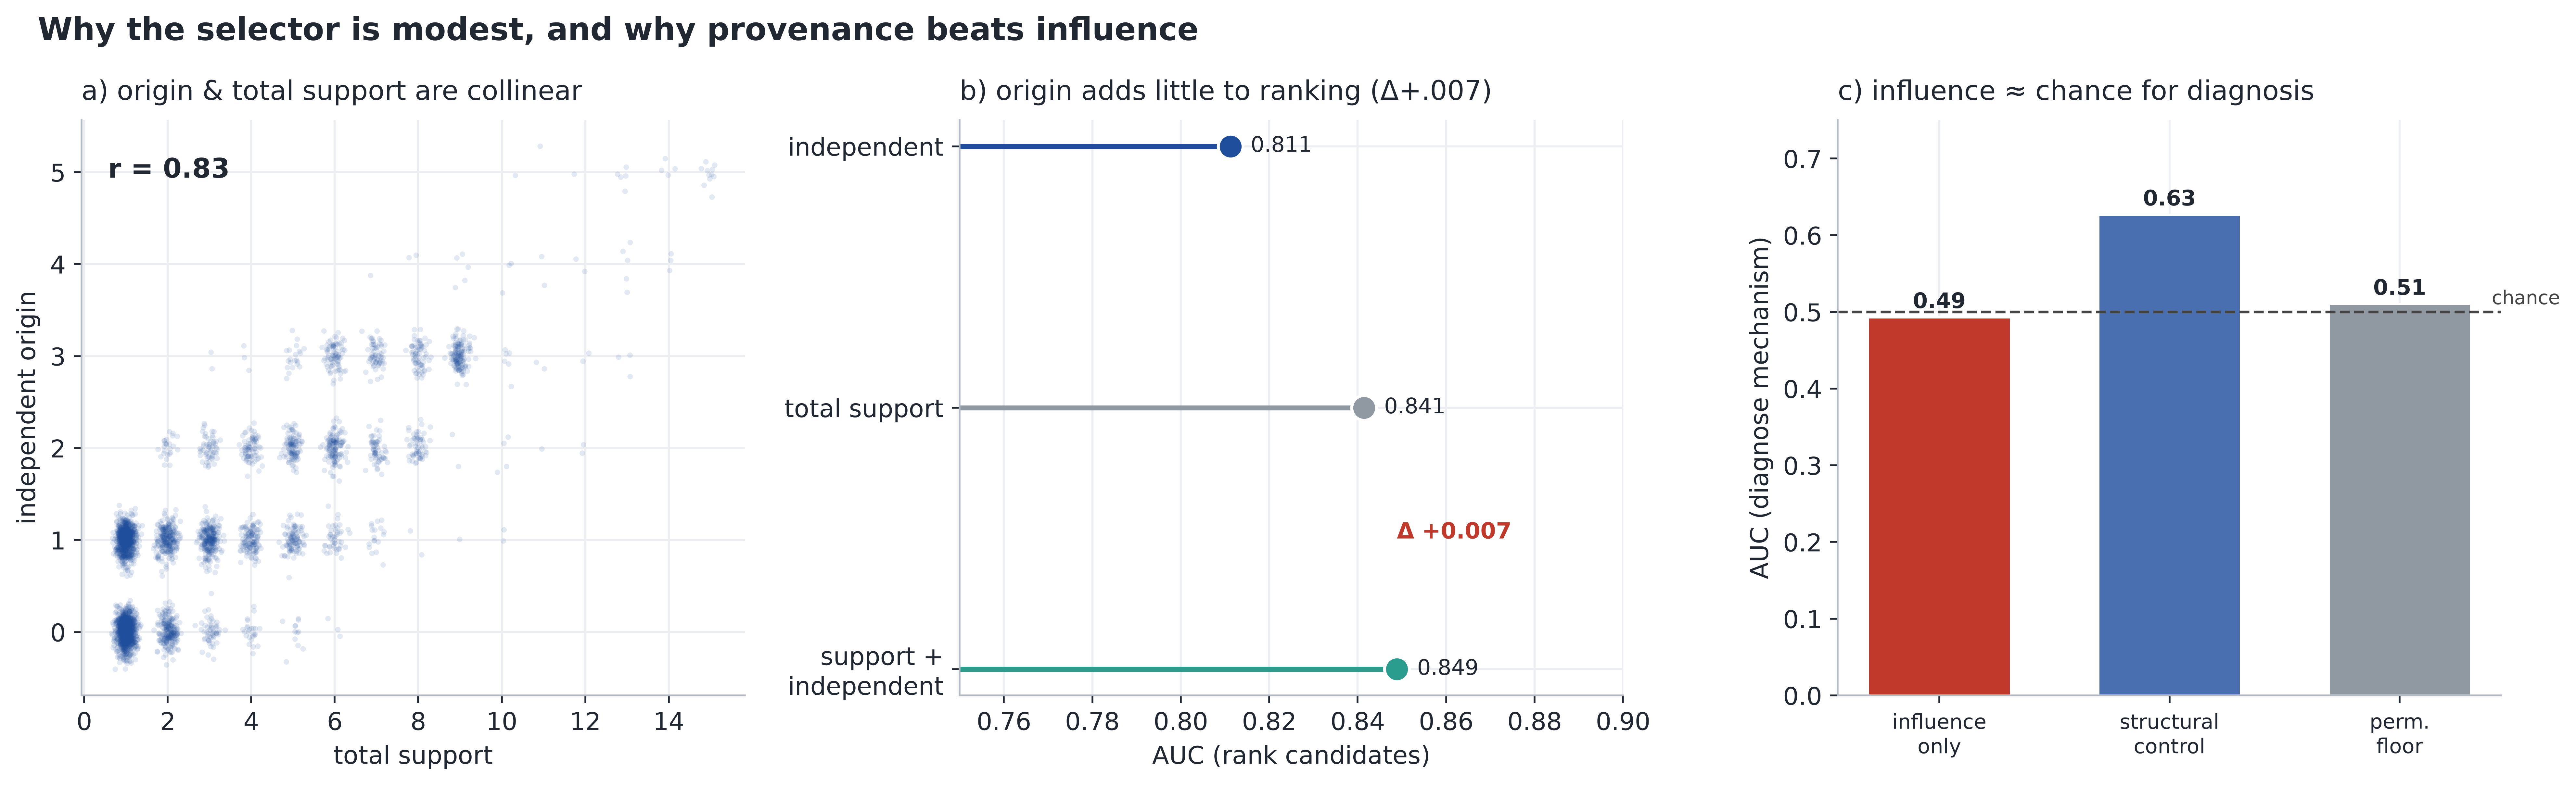
\includegraphics[width=\linewidth]{results/figures/fig9_interpretation.png}
\caption{\textbf{From influence to provenance} (referenced in \S\ref{subsec:influence_to_provenance}). Two
hypotheses can be championed by the same influential agent yet have entirely different provenance; an
agent-centric view cannot tell them apart, whereas a hypothesis-centric provenance record can. The panel
also shows why the selector is modest: origin adds little ranking power over raw consensus once they
co-vary.}
\label{fig:interpretation}
\end{figure}

\section{Failure Prediction Is Not Benefit Prediction: Full Battery}
\label{app:benefit}

\paragraph{Hazard detection and rescue.}
A round-$0$ hazard detector predicts extinction with ROC $0.757$ (LOBO $0.67$--$0.75$); detectability is
highest on StrategyQA (ROC $0.87$, lift $3.33$) and lowest on BBH, yet BBH has the largest intervention
headroom --- detectability and benefit are already decoupled. A mechanism-agnostic re-query rescues failing
debates, lifting preservation $+16$pp at matched call count.

\paragraph{Oracle and learned CATE.}
With both counterfactual arms stored, the oracle policy (target true ITE) gains $+16.5$pp pooled at a
$\sim\!20\%$ budget. A learned CATE (S- and T-learners, cross-fit over questions) predicts $Y_0$ (AUC
$0.73$) and $Y_1$ (AUC $0.67$) individually but not their difference (effect AUC $0.58$; sign
anti-correlated), so it does not beat a random budget and captures $\approx 0\%$ of the oracle gain.

\paragraph{Five pre-registered rescue attempts.}
Each attempt fixed its gate in advance (effect AUC $>0.65$ or Spearman$(\hat\tau,\mathrm{ITE})>0.20$, and a
clustered-bootstrap policy-value CI excluding zero) and changed only the feature signal: (i) cheap
structural features; (ii) residualized \textsc{nomic-embed} semantic features; (iii) an active
self-diagnosis probe (each agent names one flaw before revising); (iv) a placebo-controlled dose-response
probe; (v) the mid-debate trajectory (features observed up to rounds $1$ and $2$). All failed the gate, the
active probe nudging effect AUC only to $0.55$; the sign stayed wrong throughout. Per the pre-registered
stop rule we report the gap as the contribution.

\begin{figure}[h]
\centering
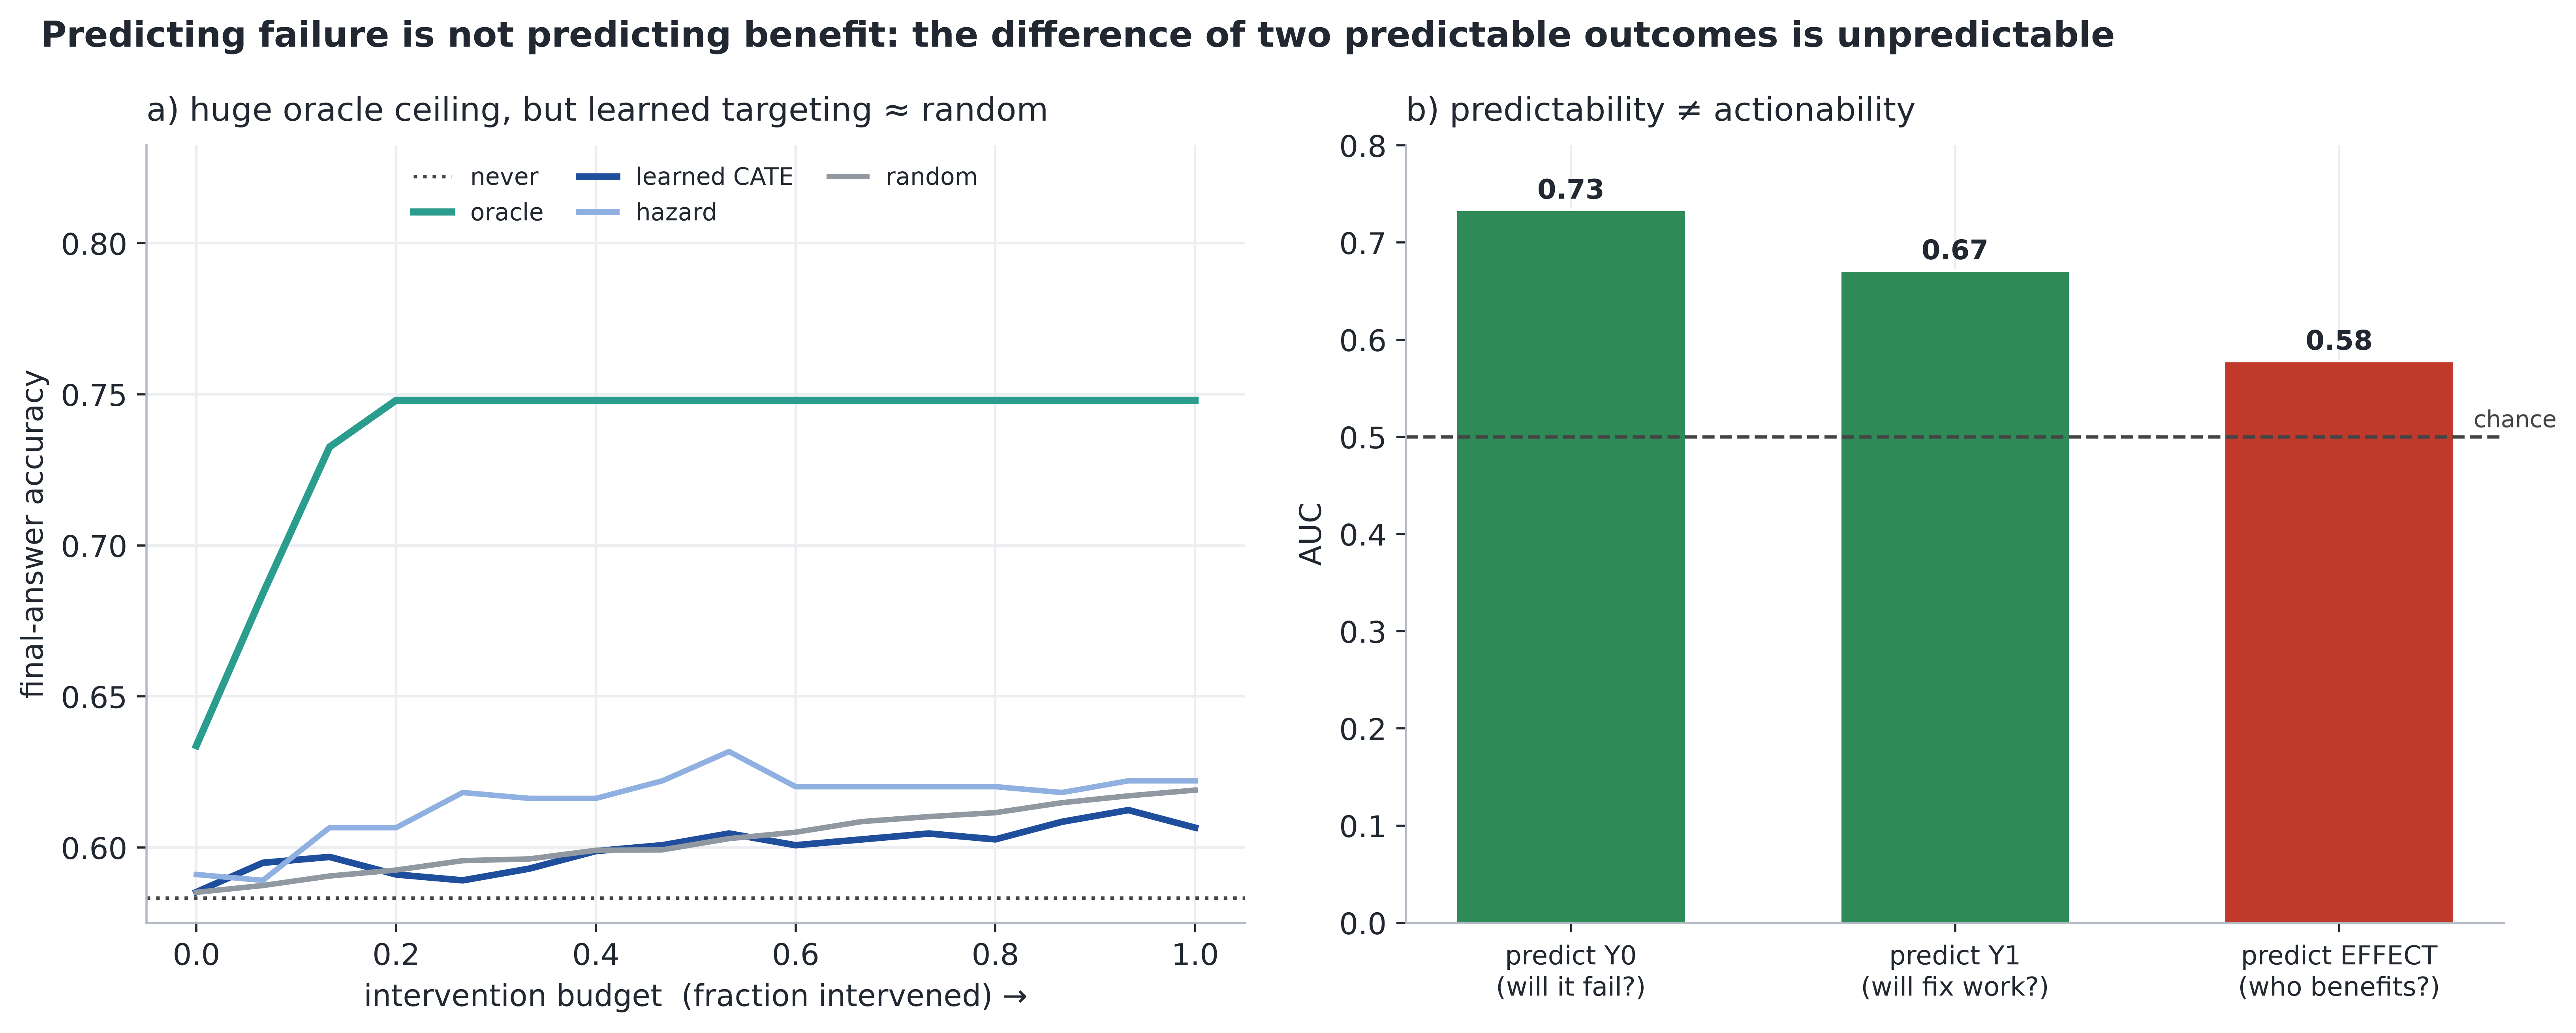
\includegraphics[width=\linewidth]{results/figures/fig12_failure_not_benefit.png}
\caption{\textbf{Failure prediction $\neq$ benefit prediction} (referenced in
\S\ref{subsec:prediction_actionability}). An oracle targeting the true treatment effect reaches the ceiling
by a $\sim\!20\%$ budget ($+16$--$20$pp), but a learned benefit predictor tracks at or below random across
five pre-registered feature families: $Y_0$ and $Y_1$ are each predictable, their difference is not.}
\label{fig:benefit}
\end{figure}

\section{Hazard-Guided Controller}
\label{app:controller}

For completeness we report the controller the conference framing would suggest. Built on the hazard
detector, it matches always-on intervention ($63.2\%$ vs.\ $62.8\%$; difference $+0.0$pp,
$[-1.6,+1.2]$) at $\sim\!55\%$ fewer interventions, but its edge over a random intervention budget is
$\approx 0$. Its one significant effect is an intervention asymmetry: it rescues $39.5\%$
$[32.4,46.8]$ of would-die debates while harming $20.6\%$ $[15.5,26.1]$ of would-live debates
(non-overlapping). Ablations show no feature group dominates and influence is not required. We demote the
controller to a supporting result because it ranks failures without converting the ranking into an accuracy
win (consistent with Appendix~\ref{app:benefit}).

\section{Provenance and Independence: Full Results}
\label{app:e26}

\paragraph{Per-benchmark origin effect.}
Table~\ref{tab:e26_bench} gives the partial coefficient $\beta_{\mathrm{ind}}$ (control total support) per
benchmark. It is significant on seven of eight; StrategyQA is the boundary.

\begin{table}[h]
\centering\small
\caption{Per-benchmark partial effect of independent support at matched total support ($\beta_{\mathrm{ind}}$;
clustered-boot $95\%$ CI).}
\label{tab:e26_bench}
\begin{tabular}{lc}
\toprule
Benchmark & $\beta_{\mathrm{ind}}$ [95\% CI] \\
\midrule
GSM8K         & $1.028\,[0.753,1.343]$ \\
CommonsenseQA & $1.179\,[0.953,1.454]$ \\
BBH           & $0.546\,[0.358,0.711]$ \\
TruthfulQA    & $0.630\,[0.375,0.890]$ \\
AQuA          & $0.752\,[0.379,1.166]$ \\
MMLU          & $0.953\,[0.686,1.261]$ \\
ARC           & $0.573\,[0.353,0.806]$ \\
StrategyQA    & $0.240\,[-0.072,0.586]$ \\
\bottomrule
\end{tabular}
\end{table}

\paragraph{Per-configuration origin effect.}
The effect holds on all five ensembles: \textsc{E\_orig} $0.684\,[0.510,0.841]$, \textsc{E\_7b}
$0.475\,[0.284,0.663]$, \textsc{E\_mixed} $1.046\,[0.851,1.218]$, \textsc{E\_strong} (14B)
$0.447\,[0.221,0.688]$, \textsc{E\_n5} ($N{=}5$) $0.304\,[0.156,0.471]$.

\paragraph{Incremental ranking power and operating points.}
Candidate-level AUC is $0.841$ for total support alone, $0.811$ for independent support alone, and $0.849$
for both --- an increment of only $+0.007$ from adding origin, quantifying the collinearity that bounds the
selector. As operating points, rejecting $n_{\mathrm{ind}}=0$ candidates removes a pool with $\Pr(\text{correct})=0.09$
(34\% coverage), and trusting $n_{\mathrm{ind}}\ge 2$ yields $\Pr(\text{correct})=0.77$ (25\% coverage).

\begin{figure}[h]
\centering
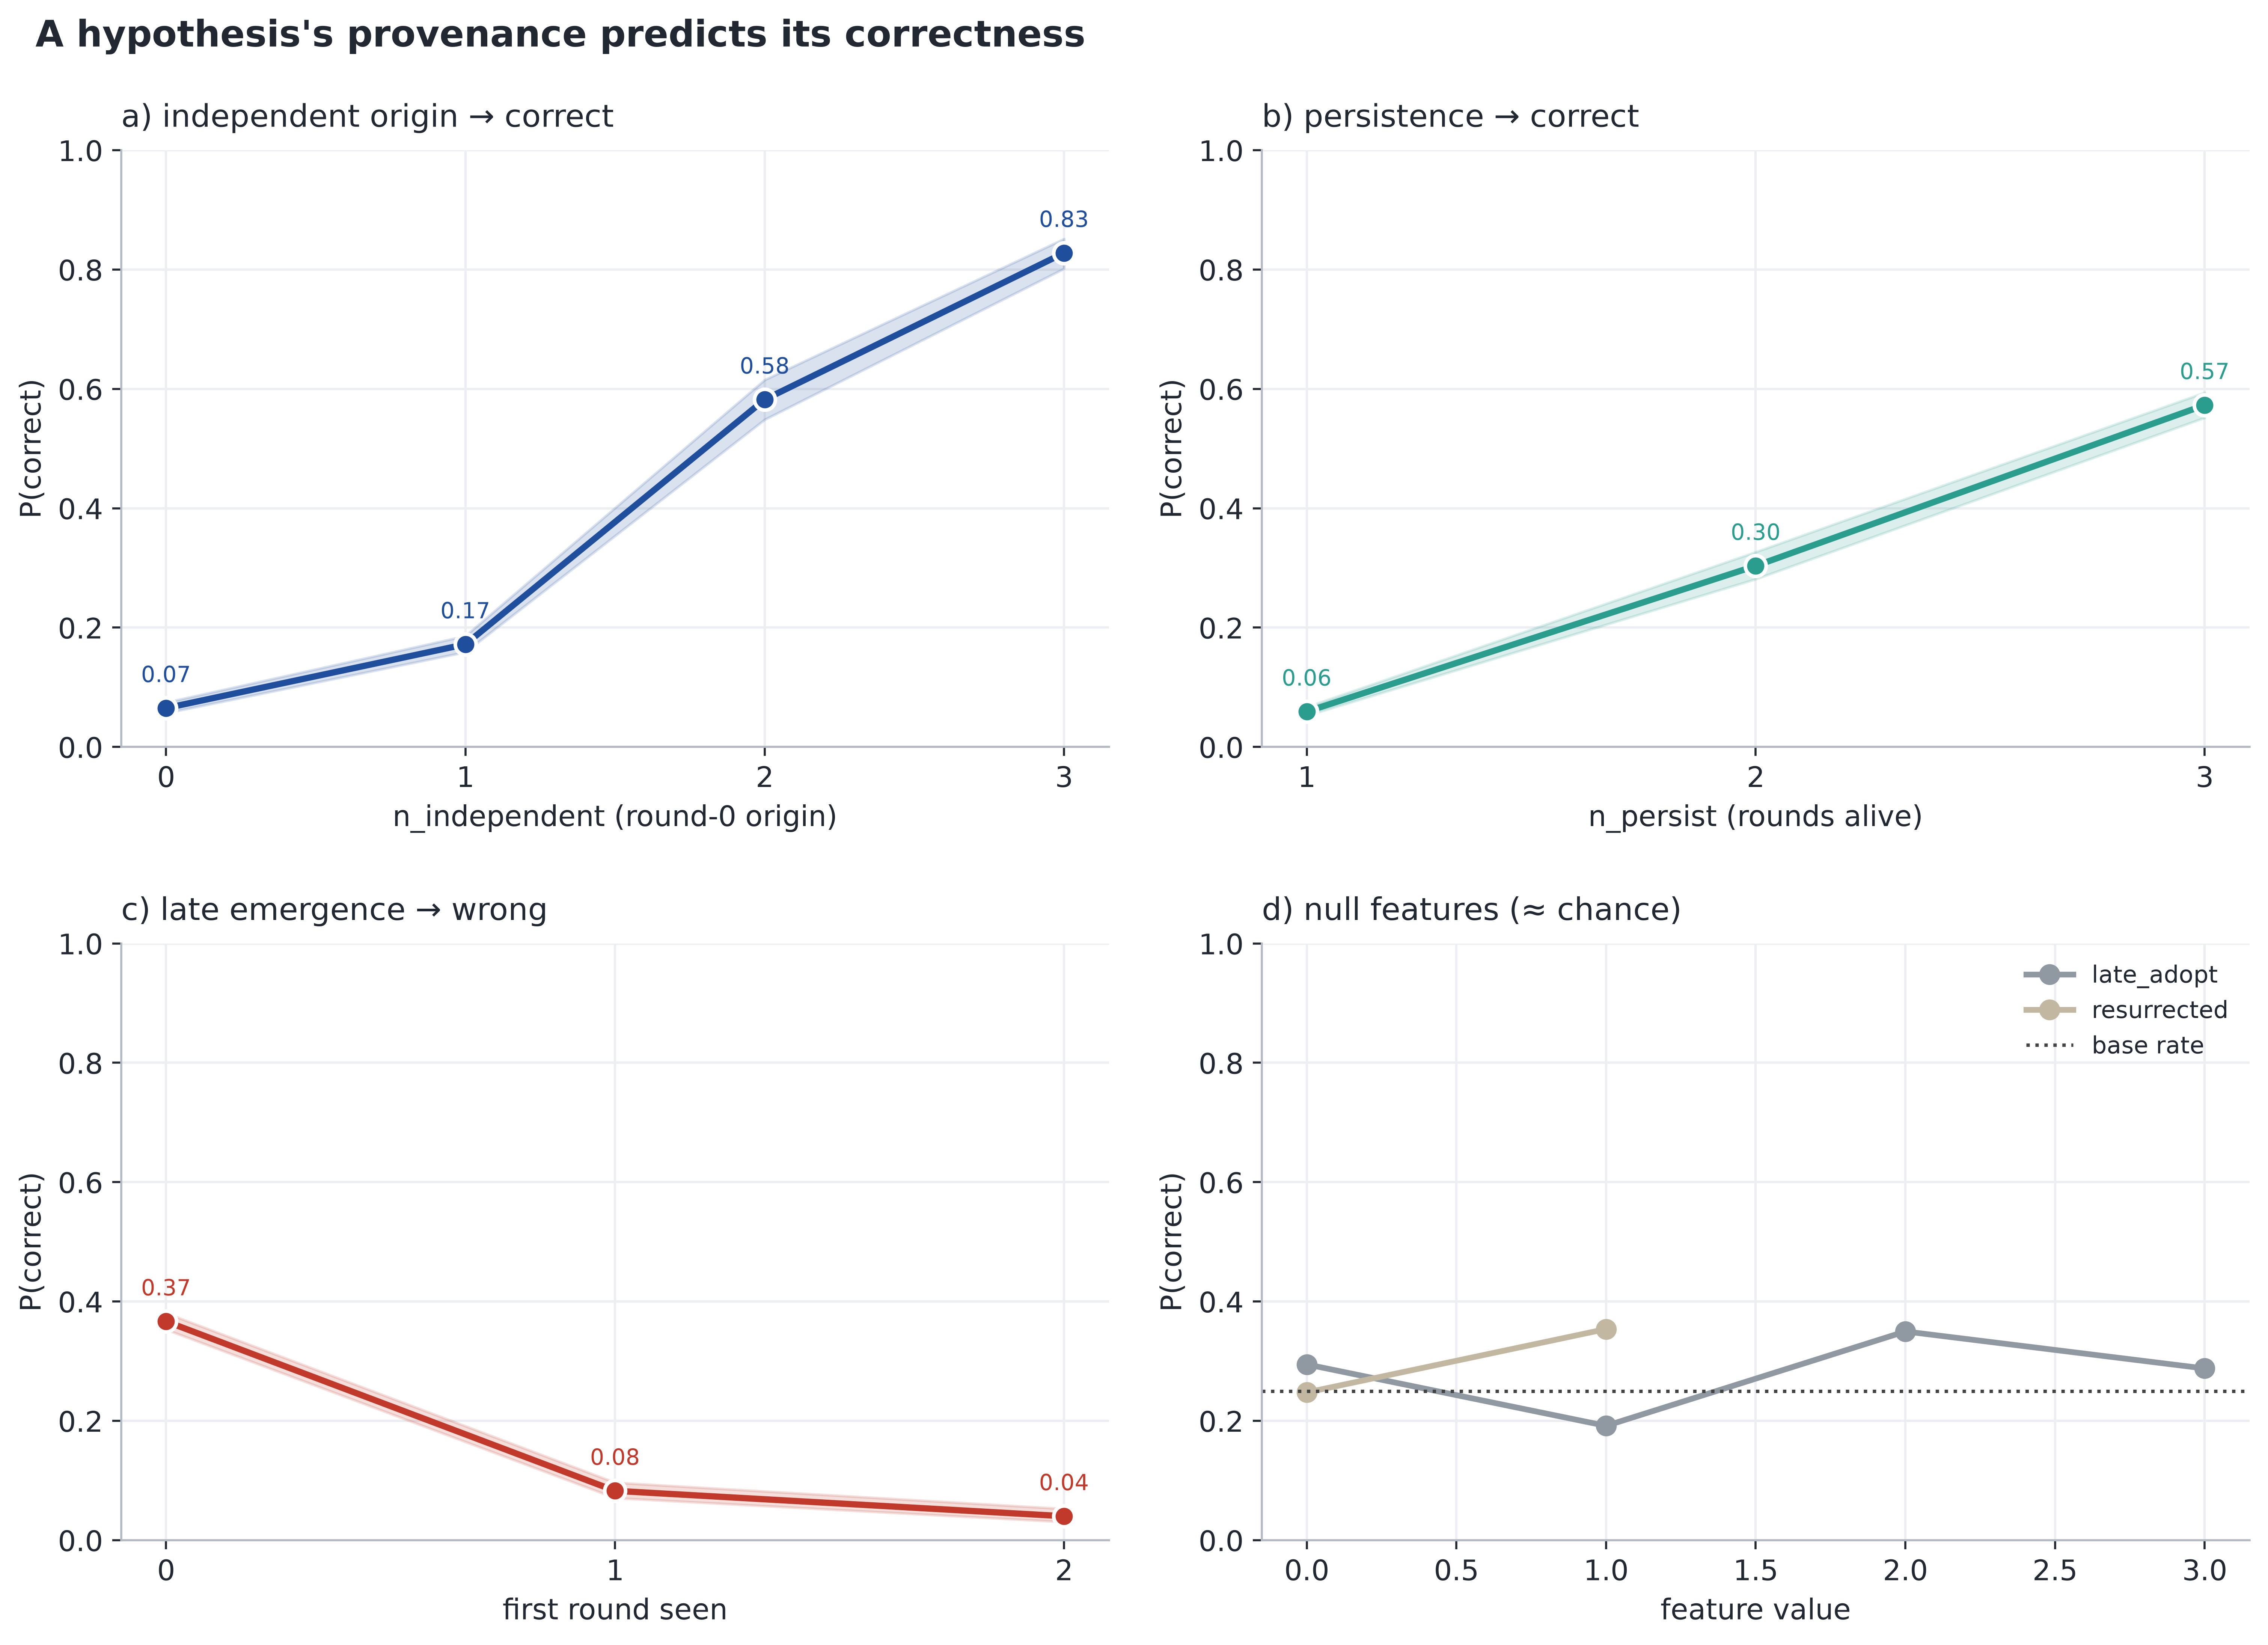
\includegraphics[width=\linewidth]{results/figures/fig3_reliability.png}
\caption{\textbf{Per-feature reliability curves} (referenced in \S\ref{subsec:provenance_correctness}).
Reliability curves for independent support and persistence climb monotonically; late-emerging hypotheses are
almost always wrong. Null features (late-adoption, resurrection) stay near the base rate.}
\label{fig:reliability}
\end{figure}

\begin{figure}[h]
\centering
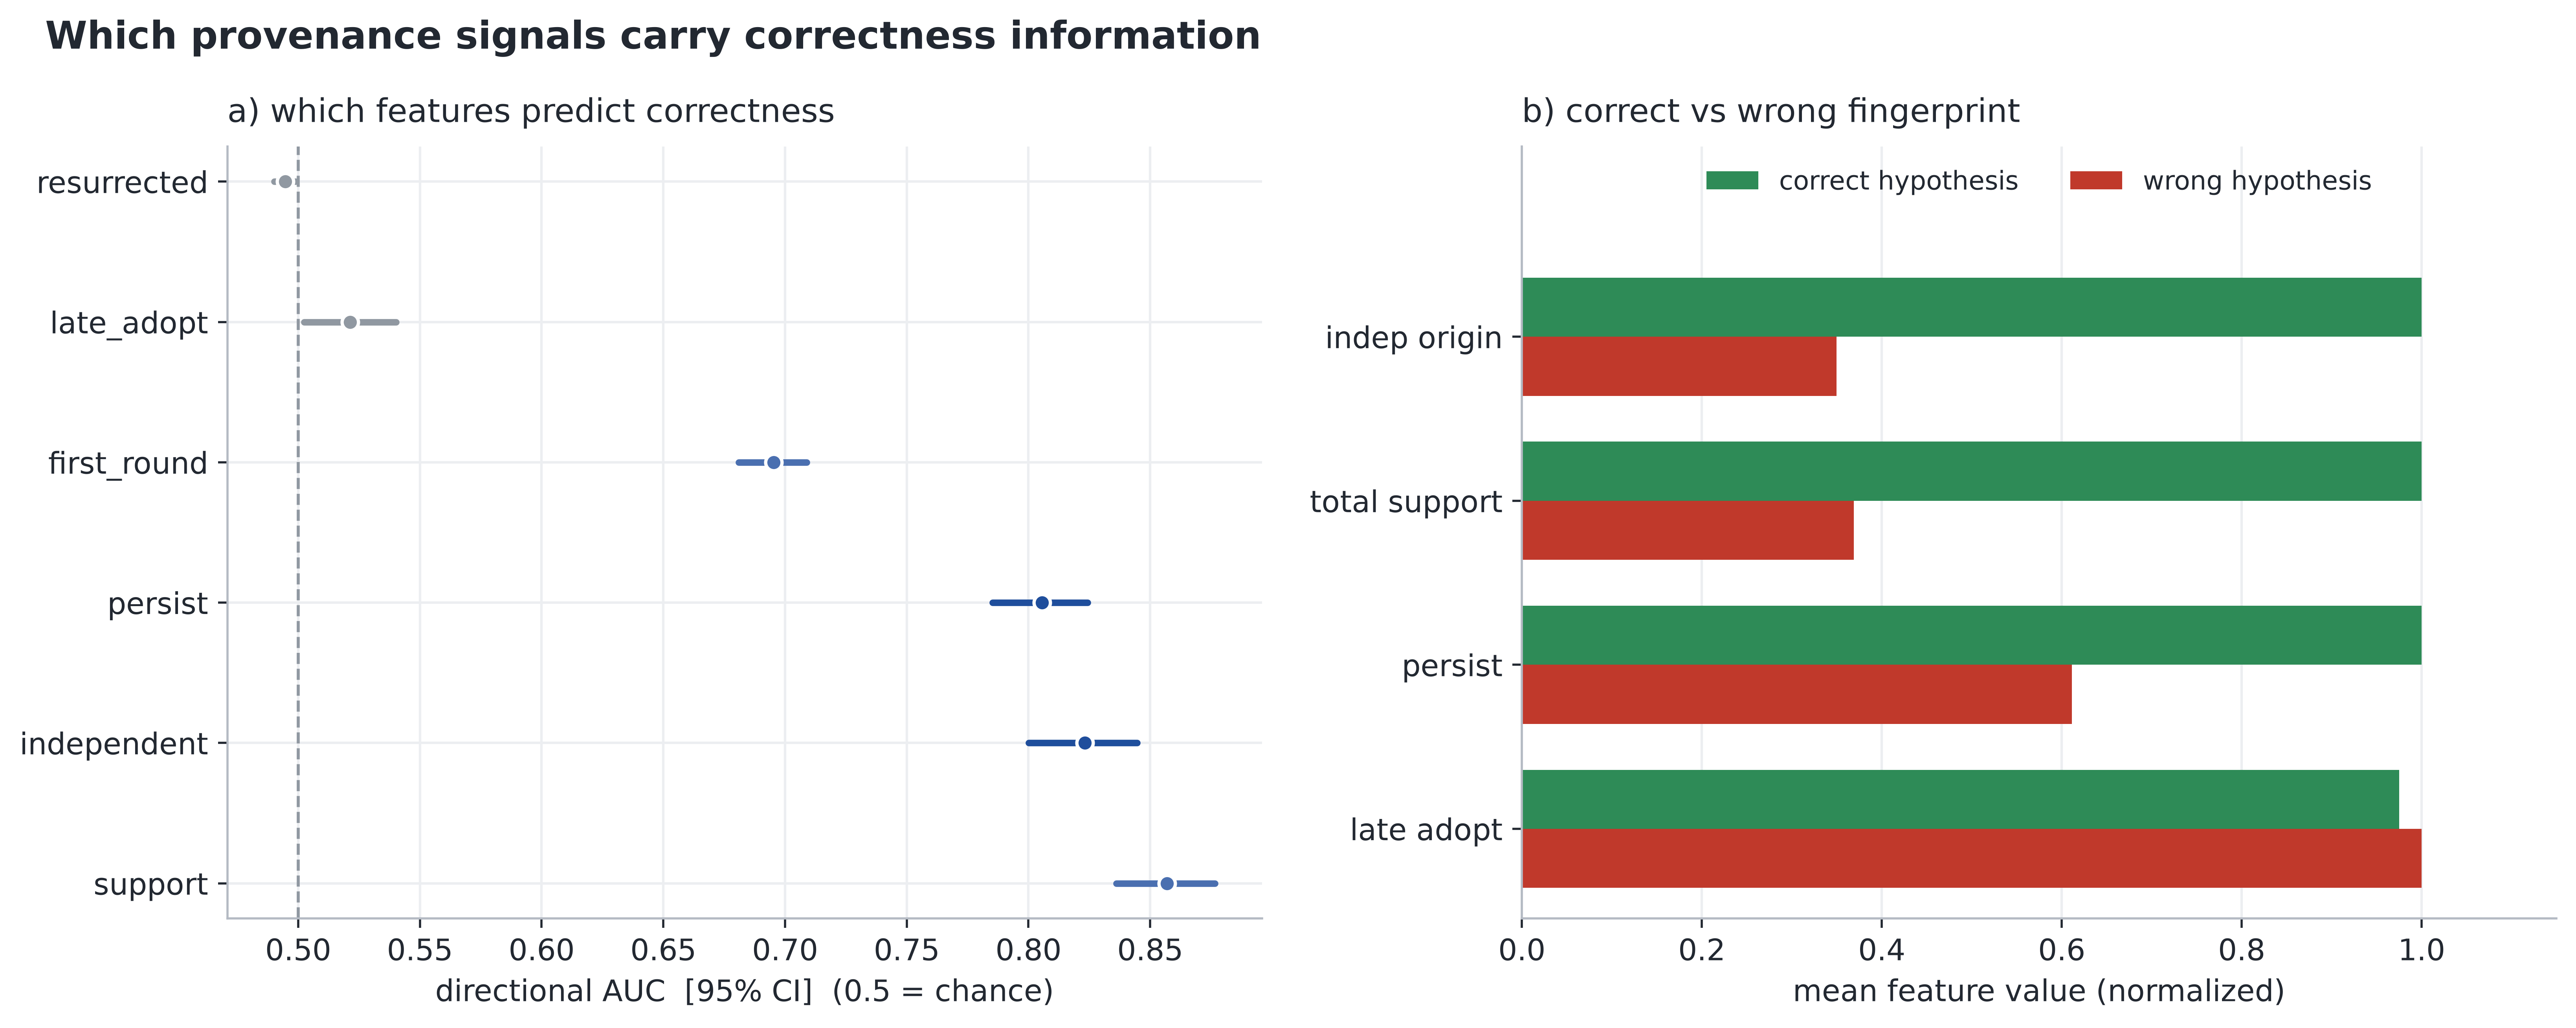
\includegraphics[width=\linewidth]{results/figures/fig4_features.png}
\caption{\textbf{Which provenance signals carry correctness information} (referenced in
\S\ref{par:provenance_comparison}). Directional AUC of each provenance feature, with the reference at
chance ($0.5$); independent support and persistence are the informative, monotone signals.}
\label{fig:features}
\end{figure}

\section{Surface versus Genuine Adoption}
\label{app:surface}

We label each social adoption \emph{genuine} if the adopter's reasoning converges toward the peer's
(lexical Jaccard residualized against the debate's baseline similarity) and \emph{surface} otherwise;
$\approx 80\%$ of adoptions are surface. A naive event-level comparison finds genuine adoptions more correct
($0.356$ vs.\ $0.292$; $\Delta=+0.064$, $[0.044,0.084]$), but a decomposition controlling for support shows
independent support towering ($\beta=1.546$) over both genuine ($0.481$) and surface ($0.495$) adoption,
whose difference is null ($-0.014$, $[-0.111,0.080]$). Origin matters; the convergence quality of later
adoption does not, once magnitude is controlled. We therefore keep this as robustness for
\S\ref{subsec:not_all_consensus_equal}, not a separate contribution.

\section{Selector Baselines, Ablations, and the External Judge}
\label{app:selectors}

\paragraph{Cheap baselines.}
Over the preserved pool, every simple gold-free selector beats the deployed majority: round-0 majority
$0.560$, anti-recency $0.558$, history frequency $0.554$, persistence $0.551$, recency $0.541$ (all CI-lo
$>0$ vs.\ majority $0.528$). This contrasts sharply with the CATE controller (Appendix~\ref{app:benefit}),
which is at chance --- selection is not blocked by the benefit-identifiability wall.

\paragraph{Deterministic arithmetic verifier.}
Selecting the pool candidate whose value equals a valid arithmetic expression in its own reasoning
\emph{hurts} versus frequency ($-0.032$ on GSM8K): correct and wrong answers are equally arithmetically
self-consistent because GSM8K errors are in problem \emph{formulation}, not computation.

\paragraph{External LLM judge.}
Forcing a judge to pick a pool label (so preservation is isolated), both a $7$B and a $14$B judge fail the
gate ($\Delta_{\mathrm{HP}}=-0.047$ and $-0.018$); the $14$B judge scores $0.76$ \emph{solving} the question
directly but only $0.53$ \emph{selecting} from the pool --- a capable external judge is a liability under
capability mismatch. StrategyQA (binary, small pool) is the lone case where judging helps.

\paragraph{Convergence-gated selector.}
Crediting late consensus only on genuine reasoning convergence recovers StrategyQA
($0.580\!\to\!0.604$) but cannot beat round-0 majority pooled, because debate is net-destructive on four of
five benchmarks and a single global rule cannot serve both regimes.

\begin{figure}[h]
\centering
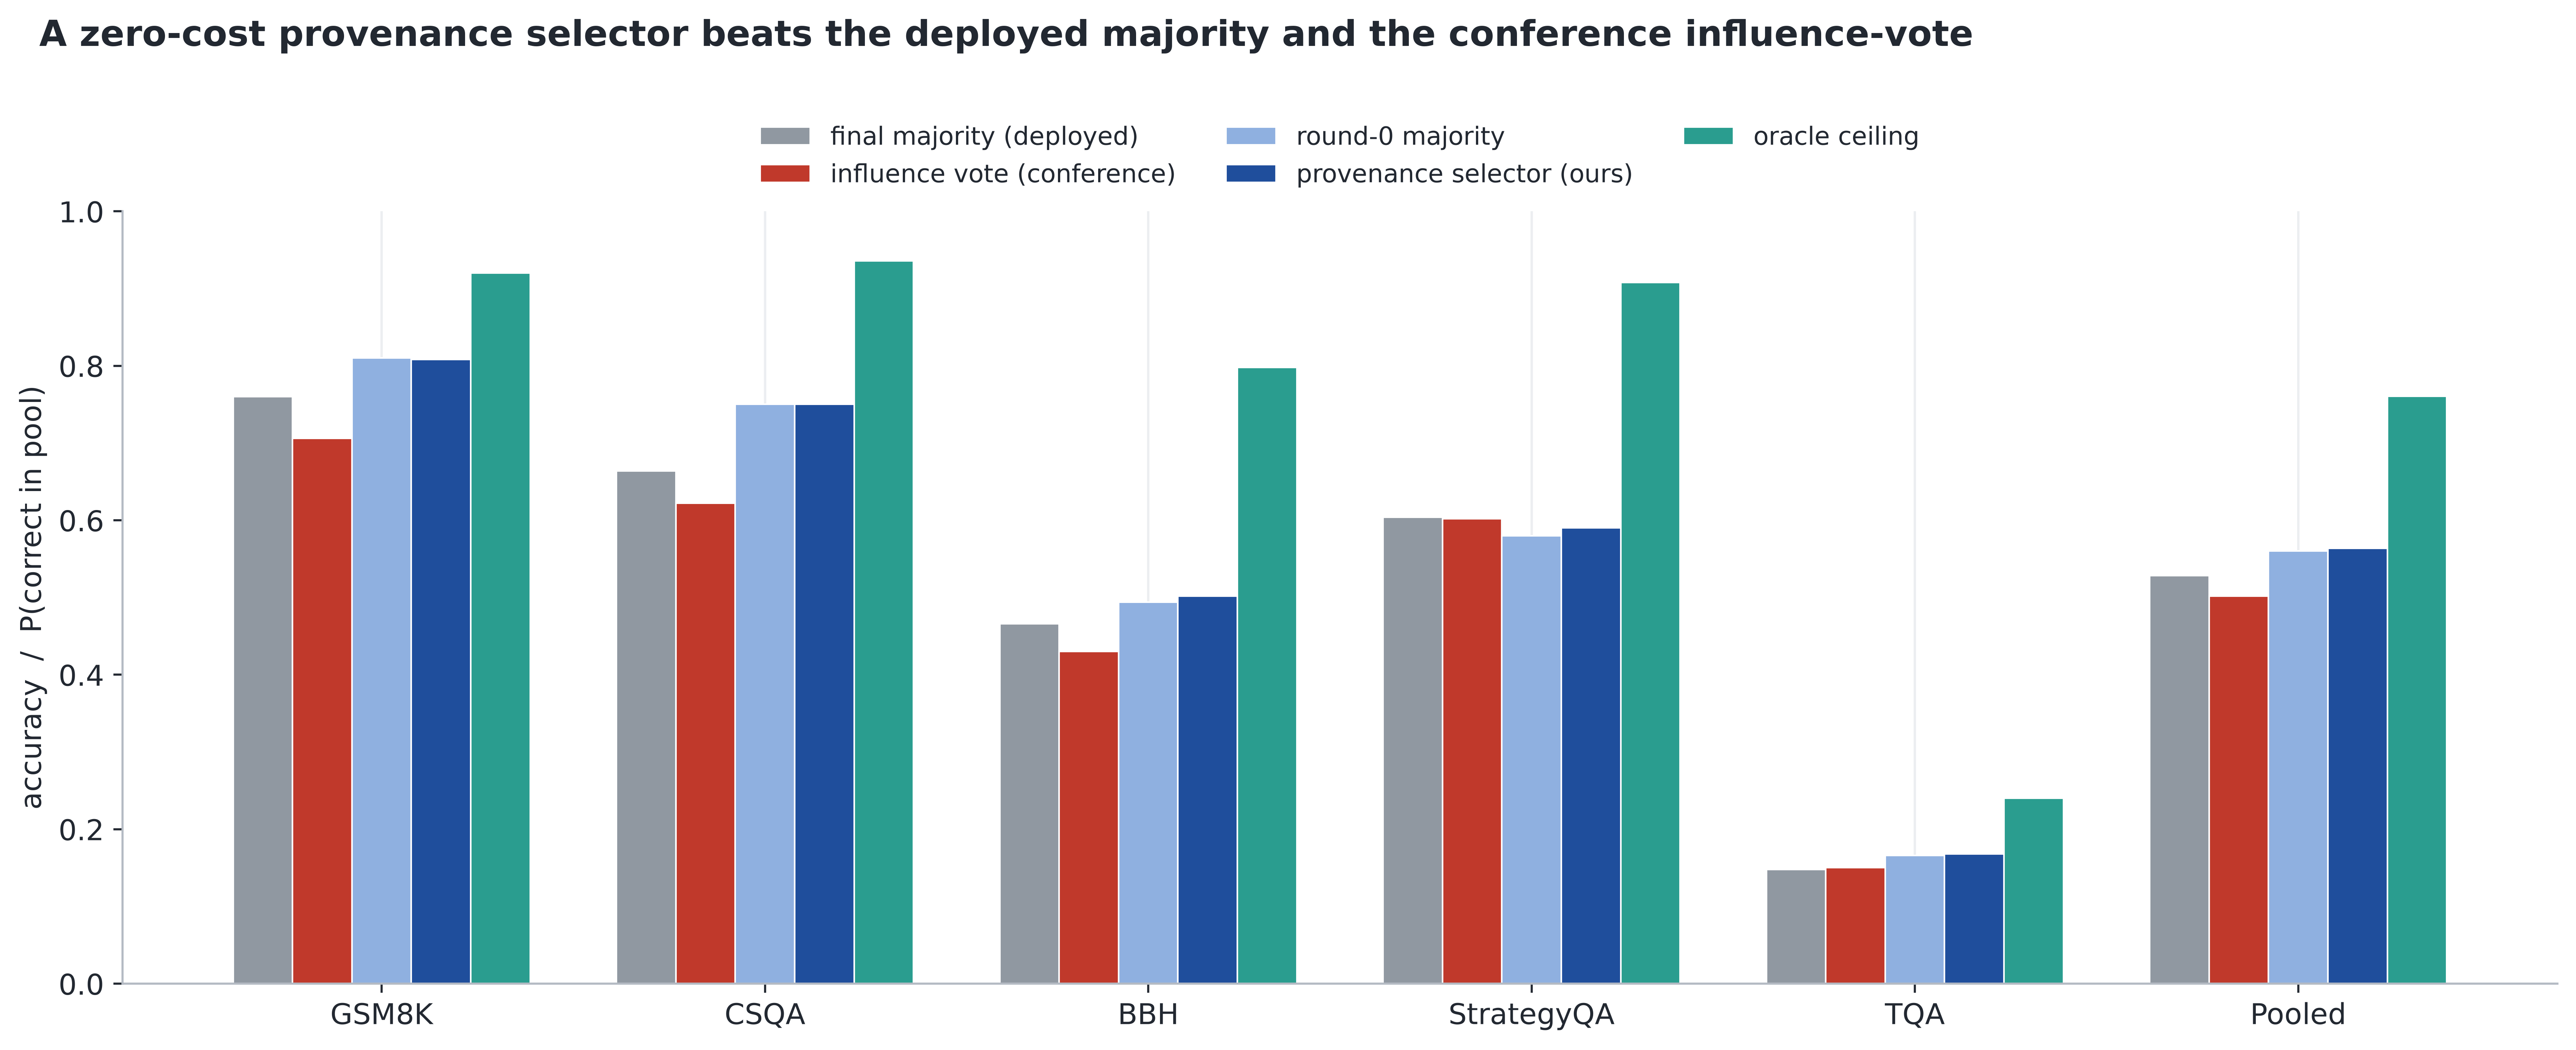
\includegraphics[width=\linewidth]{results/figures/fig11_selector_ladder.png}
\caption{\textbf{Selector ladder} (referenced in \S\ref{subsec:decision_utility}). Pooled accuracy of each
inference-time selection rule: the provenance selector beats the deployed final majority and the conference
influence vote at zero cost, while a large oracle ceiling remains. This is the graphical form of
Table~\ref{tab:selector}.}
\label{fig:ladder}
\end{figure}

\begin{figure}[h]
\centering
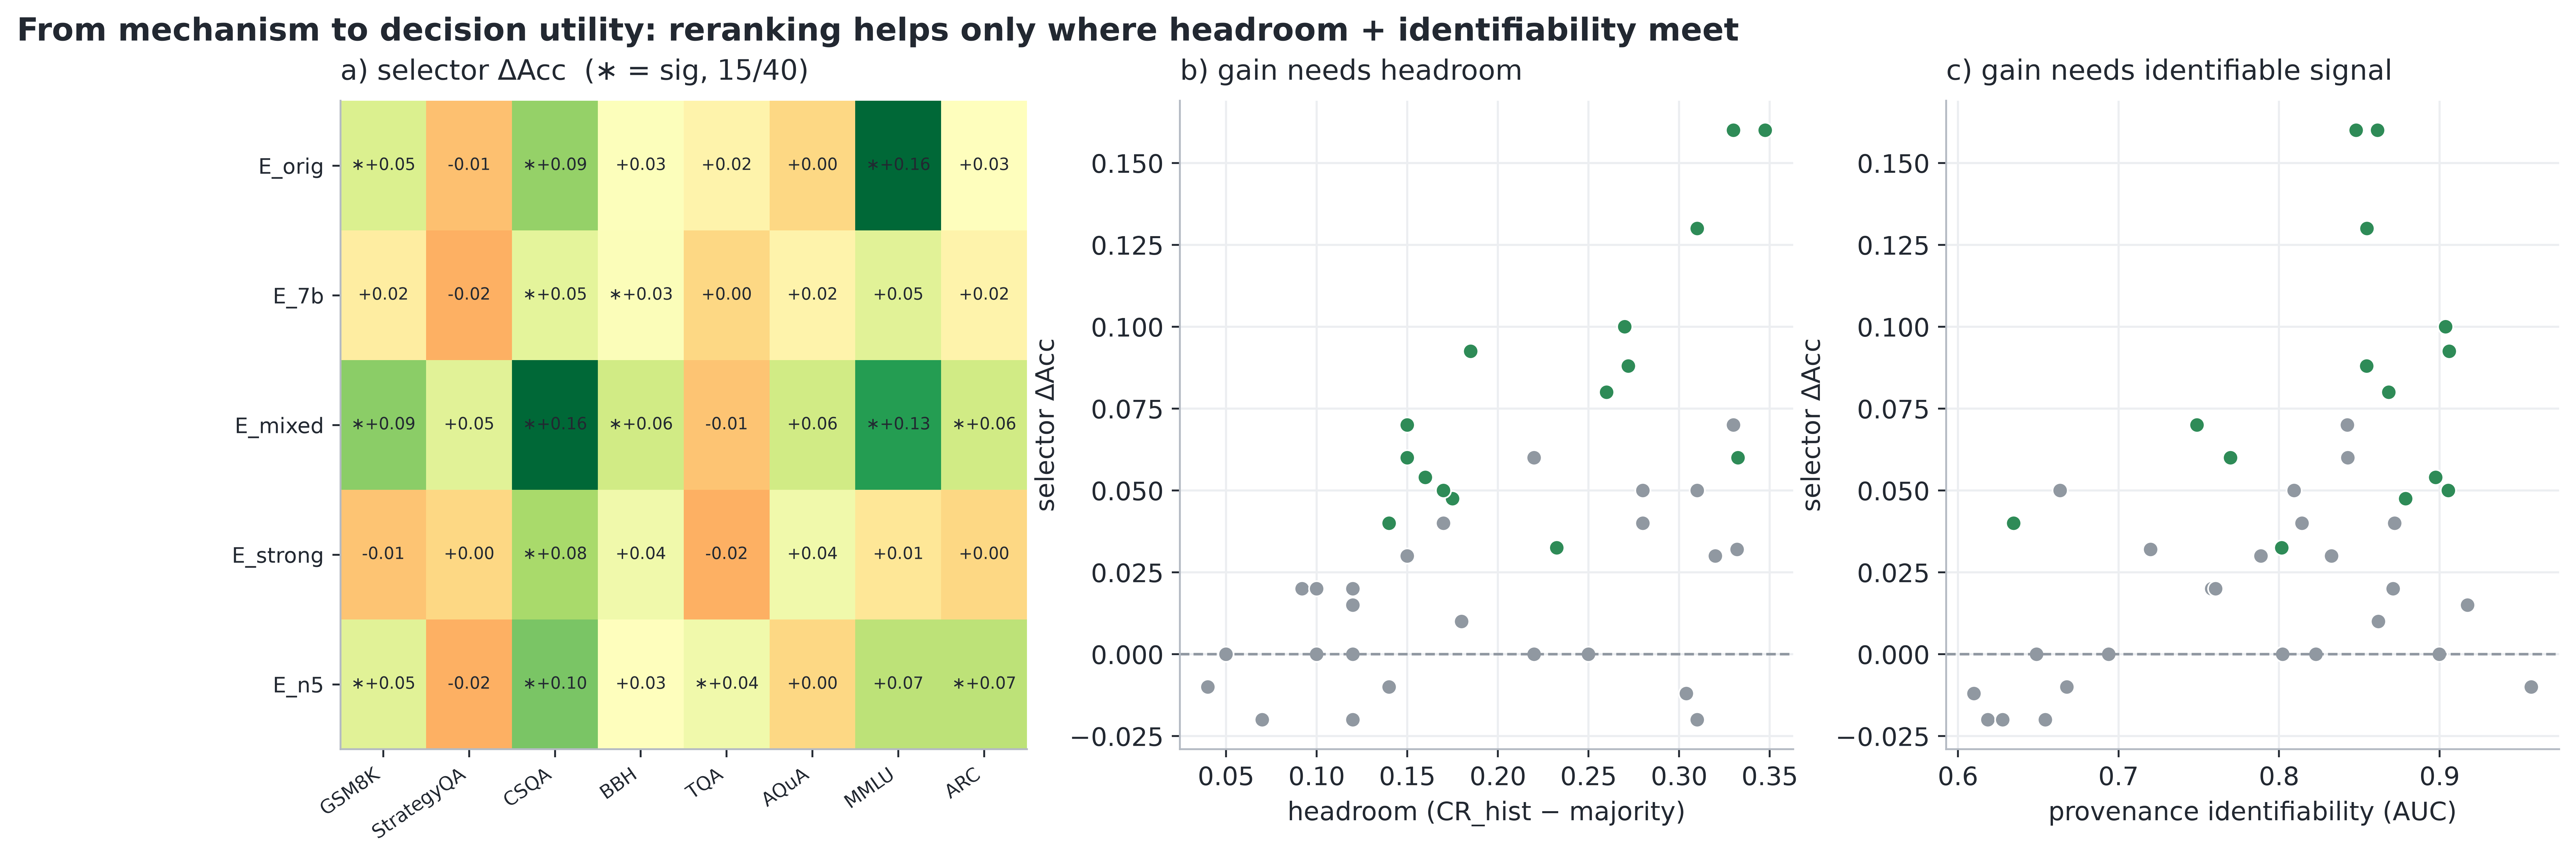
\includegraphics[width=\linewidth]{results/figures/fig8_utility.png}
\caption{\textbf{From mechanism to decision utility} (referenced in \S\ref{subsec:decision_utility}). The
provenance selector captures only $\approx 14\%$ of the preservation ceiling; its per-benchmark gain
co-varies with headroom and identifiability, and vanishes (without turning significantly negative) where
either is absent --- the applicability landscape of identifiability $\wedge$ availability.}
\label{fig:utility}
\end{figure}